\subsection{Absolutely regular or absolutely normal algebras}

DEFINITION 1.--- Let \(k\) be a field and \(A\) a \(k\)-algebra. One says that \(A\) is absolutely regular (resp. absolutely normal) \(^{1}\) if the ring \(\mathrm{A}_{(k')}\) is regular (resp. normal) for every radical extension \(k'\) of finite degree over \(k\).

Every \(k\)-algebra that is absolutely regular (resp. absolutely normal) is regular (resp. normal), as is seen by taking \(k' = k\) in Definition 1. Recall that the \(k\)-algebras A for which the ring \(\mathrm{A}_{(k')}\) is reduced for every radical extension \(k'\) of finite degree over \(k\) are the \(k\)-separable algebras (A, V, p. 117, Theorem 2).

Examples.--- 1) If k is perfect, every regular (resp. normal) k-algebra is absolutely regular (resp. absolutely normal).

\begin{enumerate}
\def\labelenumi{\arabic{enumi})}
\setcounter{enumi}{1}
\tightlist
\item
  Let A be an Artinian \(k\)-algebra. If A is normal, it is reduced, hence isomorphic to a finite product of extensions of \(k\) (A, VIII, § 8, no. 1, Proposition 2). The following conditions are equivalent:
\end{enumerate}

A is separable;

A is absolutely regular;

A is absolutely normal.

Indeed, if A is absolutely normal, it is separable; if A is separable, then for every radical extension \(k'\) of finite degree over \(k\), the ring \(\mathrm{A}_{(k')}\) is reduced and Artinian, hence isomorphic to a product of fields and consequently regular, so that \(A\) is absolutely regular.

If moreover the k-algebra A is of finite degree, the preceding conditions are equivalent to saying that A is étale (A, V, p. 34, Theorem 4).

\begin{enumerate}
\def\labelenumi{\arabic{enumi})}
\setcounter{enumi}{2}
\tightlist
\item
  Let A be a local regular \(k\)-algebra. If the extension \(\kappa_{\mathrm{A}}\) of \(k\) is separable, the algebra A is absolutely regular. Indeed, let \(k'\) be a finite extension of \(k\). The A-module \(\mathrm{A}_{(k')}\) is free. Since it is of finite type, every maximal ideal of \(\mathrm{A}_{(k')}\) lies over \(\mathfrak{m}_{\mathrm{A}}\) (V, § 2, no. 1, Proposition 1). The ring \(\kappa_{\mathrm{A}} \otimes_{\mathrm{A}} \mathrm{A}_{(k')}\), isomorphic to \(\kappa_{\mathrm{A}} \otimes_{k} k'\), is regular (no. 3, Lemma 2). By the corollary of Proposition 9 of § 4, no. 5, the ring \(\mathrm{A}_{(k')}\) is regular, which proves that the \(k\)-algebra A is absolutely regular.
\end{enumerate}

PROPOSITION 6. Let k be a field and A a Noetherian k-algebra.

\begin{enumerate}
\def\labelenumi{\alph{enumi})}
\item
  If A is absolutely regular (resp. absolutely normal, resp. separable), then so is \(S^{-1}A\) for every multiplicative subset S of A.
\item
  If \(A_{m}\) is absolutely regular (resp. absolutely normal, resp. separable) for every maximal ideal m of A, then A is absolutely regular (resp. absolutely normal, resp. separable).
\item
  This follows from the fact that the ring \((\mathrm{S}^{-1}\mathrm{A})_{(k^{\prime})}\) is isomorphic to a ring of fractions of the ring \(\mathrm{A}_{(k^{\prime})}\) for every extension \(k^{\prime}\) of k.
\item
  Suppose that \(A_{m}\) is absolutely regular (resp. absolutely normal, resp. separable) for every maximal ideal m of A. Let \(k'\) be a radical extension of k of finite degree and let \(m'\) be a maximal ideal of \(\mathrm{A}_{(k')}\). It remains to verify that the local ring \((\mathrm{A}_{(k')})_{\mathfrak{m}'}\) is regular (resp. normal, resp. reduced).
\end{enumerate}

The canonical homomorphism \(A \to A_{(k')}\) makes \(A_{(k')}\) into a finite A-algebra. The ideal \(m'\) lies over a maximal ideal m of A (V, § 2, no. 1, Proposition 1), and \((\mathrm{A}_{(k')})_{\mathfrak{m}'}\) is isomorphic to a ring of fractions of the regular (resp. normal, resp. reduced) ring \((\mathrm{A}_{\mathfrak{m}})_{(k')}\), hence is regular (resp. normal, resp. reduced).

Lemma 3.--- Let k be a field and K a finitely generated extension of k. There exists an extension L of K, of finite degree, and a subextension k' of L over k, radical and of finite degree over k, such that the extension L of k' is separable.

Choose a composite extension E of K and of a perfect closure \(\hat{k}\) of \(k\), and elements \((t_1, \ldots, t_n)\) of E such that E is a separable algebraic extension of \(\hat{k}(t_1, \ldots, t_n)\). Let I be a finite generating set of K over \(k\). The field \(\hat{k}(t_1, \ldots, t_n)\) (resp. \(\hat{k}\mathrm{K}\)) is the union of the subfields \(k'(t_1, \ldots, t_n)\) (resp. \(k'\mathrm{K}\)), where \(k'\) ranges over the set of subextensions of \(\hat{k}\) of finite degree over \(k\); one can therefore find such a subextension \(k'\) such that the elements \(t_1, \ldots, t_n\) of \(\mathrm{E} = \hat{k}\mathrm{K}\) belong to \(k'\mathrm{K}\) and each element of I is algebraic and separable over \(k'(t_1, \ldots, t_n)\). Then \(\mathrm{L} = k'\mathrm{K}\) is a separable extension of \(k'\) of finite degree over K, and \(k'\) is a radical extension of finite degree over \(k\).

PROPOSITION 7. Let \(k\) be a field, and let A and B be \(k\)-algebras, one of which is essentially of finite type. Suppose that A is absolutely regular (resp. absolutely normal). If the ring B is regular (resp. normal), then so is the ring A \(\otimes_{k}\) B.

Let K be a finitely generated extension of k; let us prove that the ring \(\mathrm{A}_{(\mathrm{K})}\) is regular (resp. normal). Indeed, consider extensions L and \(k'\) having the properties of Lemma 3. Then the ring \(\mathrm{A}_{(k')}\) is regular (resp. normal) by definition, and the ring \(\mathrm{A}_{(\mathrm{L})}\), which is identified with \(\mathrm{A}_{(k')} \otimes_{k'} \mathrm{L}\), is regular (resp. normal) by Proposition 5, b) of No. 3. Consequently, \(\mathrm{A}_{(\mathrm{K})}\) is regular (resp. normal) by Proposition 5, a).

Suppose the ring B is regular (resp. normal) and let us prove the proposition. The canonical homomorphism \(B \to A \otimes_{k} B\) makes \(A \otimes_{k} B\) a free B-module. For every prime ideal p of B, the ring \((A \otimes_{k} B) \otimes_{B} \kappa(\mathfrak{p})\) is identified with \(A \otimes_{k} \kappa(\mathfrak{p})\) by the corollary of Proposition 9 of § 4, No. 5 (resp. Corollary 3 of Theorem 4 of § 1, No. 10); it suffices for us to prove that \(A \otimes_{k} \kappa(\mathfrak{p})\) is regular (resp. normal) for every prime ideal p of B.

If the \(k\)-algebra B is essentially of finite type, the extension \(\kappa(\mathfrak{p})\) of \(k\) is of finite type and the ring A \(\otimes_k \kappa(\mathfrak{p})\) is regular (resp. normal) by what we saw above. Now suppose the \(k\)-algebra A is essentially of finite type; the ring A \(\otimes_k \kappa(\mathfrak{p})\) is Noetherian and is the union of the increasing filtered family of Noetherian subrings \(A \otimes_k K\), where \(K\) runs through the finitely generated subextensions of \(\kappa(\mathfrak{p})\). These latter rings are regular (resp. normal), and one applies Lemma 1 of No. 3.

COROLLARY 1. Let k be a field. The tensor product of two absolutely regular (resp. absolutely normal) k-algebras, one of which is essentially of finite type, is an absolutely regular (resp. absolutely normal) k-algebra.

Let A and B be two k-algebras satisfying the hypotheses of the corollary. Let \(k'\) be a radical extension of k of finite degree. The ring \(\mathrm{B}_{(k')}\) is regular (resp. normal); the ring \(A \otimes_{k} B_{(k')}\) is regular (resp. normal) by prop. 7, as is the ring \((\mathrm{A} \otimes_{k} \mathrm{B}) \otimes_{k} k'\) which is isomorphic to it.

COROLLARY 2.--- Let k be a field, A an absolutely regular (resp. absolutely normal) k-algebra, and K an extension of k. Suppose that A is essentially of finite type or that the extension K of k is of finite type.

\begin{enumerate}
\def\labelenumi{\alph{enumi})}
\item
  The ring \(\mathrm{A}_{(K)}\) is regular (resp. normal).
\item
  If the extension K of k is separable, the k-algebra \(\mathrm{A}_{(\mathrm{K})}\) is absolutely regular (resp. absolutely normal).
\end{enumerate}

Assertion (a) follows from Proposition 7; assertion (b) follows from Corollary 1 and Example 2.

COROLLARY 3. Let \(k\) be a field, let A be a \(k\)-algebra, and let K be an extension of \(k\). Suppose that the \(k\)-algebra A is essentially of finite type or that the extension K of \(k\) is of finite type. For the \(k\)-algebra A to be absolutely regular (resp. absolutely normal), it is necessary and sufficient that the K-algebra \(\mathrm{A}_{(\mathrm{K})}\) be absolutely regular (resp. absolutely normal).

Suppose A is absolutely regular (resp. absolutely normal) and let \(K'\) be a radical extension of K of finite degree. The ring \(K'\otimes_{K}A_{(K)}\), which is isomorphic to \(K'\otimes_{k}A\), is regular (resp. normal) by Corollary 2.

Conversely, suppose the K-algebra \(\mathrm{A}_{(\mathrm{K})}\) is absolutely regular (resp. absolutely normal) and let \(k'\) be a radical extension of \(k\) of finite degree. Let L be a composite extension of \(k'\) and K; then the ring \(\mathrm{A}_{(\mathrm{L})}\) is identified with \(\mathrm{L} \otimes_{\mathrm{K}} \mathrm{A}_{(\mathrm{K})}\), hence is regular (resp. normal); consequently, the ring \(\mathrm{A}_{(k')}\) is regular (resp. normal) by Proposition 5, a) of No. 3.

COROLLARY 4.--- Let k be a field, A a k-algebra essentially of finite type, and K an extension of k which is a perfect field. For A to be absolutely regular (resp. absolutely normal), it is necessary and sufficient that the ring \(\mathrm{A}_{(\mathrm{K})}\) be regular (resp. normal).

This follows from Cor. 3 and Example 1.

\subsection{Characterizations of absolutely regular algebras}

PROPOSITION 8. Let \(k\) be a field and let A be an essentially of finite type \(k\)-algebra. Let I denote the kernel of the homomorphism of \(k\)-algebras \(\mu: A \otimes_k A \to A\) such that \(\mu(x \otimes y) = xy\) for \(x\) and \(y\) in A. The following conditions are equivalent:

\begin{enumerate}
\def\labelenumi{(\roman{enumi})}
\item
  the k-algebra A is absolutely regular;
\item
  for every regular k-algebra C, the ring A ⊗k C is regular;
\item
  the ring A ⊗k A is regular;
\item
  the ideal I of A ⊗k A is completely secant (§ 5, no. 1, def. 1).
\end{enumerate}

Let B denote the ring A \(\otimes_{k}\) A and endow it with the structure of an A-algebra deduced from the homomorphism \(\rho: \mathrm{A} \to \mathrm{A} \otimes_{k} \mathrm{A}\) such that \(\rho(x) = x \otimes 1\); then \(\mu\) is a homomorphism of A-algebras and induces, by passage to the quotient, an isomorphism from B/I onto A.

(i)⇒(ii): this follows from Proposition 7.

(ii)⇒(iii): it suffices to apply (ii) with C=k, then with C=A.

(iii)⇒(iv): the A-module B is free, hence faithfully flat. If the ring B is regular, then A is regular (§ 4, no. 5, prop. 8); the ideal I is then completely secant (§ 5, no. 3, prop. 2).

(iv)⇒(i): suppose the ideal I is completely secant and first prove that A is regular. Let m be a maximal ideal of A and let \(\nu:(\mathrm{A}/\mathfrak{m})\otimes_{k}\mathrm{A}\to\mathrm{A}/\mathfrak{m}\) be the homomorphism deduced from \(\mu\). The maximal ideal n=Ker \(\nu\) is equal to \(I((\mathrm{A}/\mathfrak{m})\otimes_{k}A)\); applying Proposition 6 of § 5, No. 6, to the A-algebra \(A'=A/\mathfrak m\), we see that the ideal n is completely secant in \((A/\mathfrak{m})\otimes_{k}A\). Consequently (§ 5, No. 3, Proposition 3), the local ring \(((\mathrm{A}/\mathfrak{m})\otimes_{k}A)_{n}\) is regular. Denote \(j:\mathrm{A}\to(\mathrm{A}/\mathfrak{m})\otimes_{k}\mathrm{A}\) the homomorphism \(x\mapsto1\otimes x\); since \(\nu\circ j\) is the canonical homomorphism from A to A/m, we have \(j^{-1}(\mathfrak{n})=\mathfrak{m}\). Thus j extends to a local homomorphism of local rings from \(A_{m}\) into \(((\mathrm{A}/\mathfrak{m})\otimes_{k}\mathrm{A})_{n}\), which makes the latter an \(A_{m}\)-module that is faithfully flat. By Proposition 8 of § 4, No. 5, the ring \(A_{m}\) is therefore regular. We have thus proved that A is regular.

Now let \(k'\) be an extension of \(k\). The kernel of the map \(\mu': A_{(k')} \otimes_{k'} A_{(k')} \to A_{(k')}\) deduced from the multiplication of \(A_{(k')}\) is none other than \(IA_{(k')}\); it is therefore completely secant in \(A_{(k')}\) (§ 5, No. 6, Proposition 6). The \(k'\)-algebra \(A_{(k')}\) therefore satisfies condition (iv); by what has just been seen, it is regular, and this proves (i).

Recall (A, III, pp. 133–134) that the quotient I/I², endowed with the A-module structure induced by ρ, is denoted Ωₖ(A) and called the module of k-differentials of A. When the k-algebra A is essentially of finite type, the ring A ⊗ₖ A is Noetherian, so that the A-module Ωₖ(A) is finitely generated.

One denotes by \(d_{A/k}\) or simply \(d\) the \(k\)-linear map from A into \(\Omega_k(A)\) which associates to an element \(x\) of A the class of \(x \otimes 1 - 1 \otimes x\) in \(\Omega_k(A)\). The map \(d\) is a \(k\)-derivation; for every A-module M and every \(k\)-derivation D: A → M, there exists a unique A-linear map \(g: \Omega_k(A) \to M\) such that D = g ∘ d (loc. cit., Proposition 18).

If S is a multiplicative subset of A, the canonical \(S^{-1}A\)-linear map (loc. cit., p. 136)

\[
\mathrm{S} ^ {- 1} \Omega_ {k} (\mathrm{A}) \rightarrow \Omega_ {k} (\mathrm{S} ^ {- 1} \mathrm{A})
\]

is bijective: indeed, it suffices to verify that, for every S \(^{-1}\) A-module M, every k-derivation D : A → M extends uniquely to a k-derivation D : S \(^{-1}\) A → M; this follows from the argument of loc. cit., p. 123, Proposition 5.

Let \(k\) be a field and A a local, essentially of finite type \(k\)-algebra. Set \(n = \dim(A) + \deg.\mathrm{tr}_k(\kappa_A)\). Let B be a finitely generated \(k\)-algebra and \(\mathfrak{q}\) a prime ideal of B such that the \(k\)-algebra A is isomorphic to \(\mathbf{B}_{\mathfrak{q}}\) (\(cf.\ n^{\circ} 1\), Example 2); we have \(n = \dim_{\mathfrak{q}}(\mathbf{B})\) (VIII, § 2, no. 4, Corollary 5 of Theorem 3). By loc. cit., Theorem 3, c) and Corollary 5, we also have

\[
n = \sup \deg . \operatorname{tr} _ {k} (\kappa (\mathfrak {p}))
\]

where p ranges over the finite family of minimal prime ideals of A. If A is integral, n is therefore the transcendence degree of the field of fractions of A.

THEOREM 1. Let \(k\) be a field and A a local, essentially of finite type \(k\)-algebra. Set \(n = \dim(A) + \deg.\mathrm{tr}_{k}(\kappa_{A})\).

\begin{enumerate}
\def\labelenumi{\alph{enumi})}
\item
  One has \([\kappa_{A} \otimes_{A} \Omega_k(A): \kappa_{A}] \geqslant n\).
\item
  The following conditions are equivalent:
\end{enumerate}

\begin{enumerate}
\def\labelenumi{(\roman{enumi})}
\item
  the k-algebra A is absolutely regular;
\item
  the A-module \(\Omega_{k}(\mathrm{A})\) is free of rank \(n\);
\end{enumerate}

\[
\left[ \kappa_ {A} \otimes_ {A} \Omega_ {k} (A): \kappa_ {A} \right] = n
\]

Consider the assertion

(iii') one has \([\kappa_{\mathrm{A}} \otimes_{A} \Omega_k(\mathrm{A}):\kappa_{\mathrm{A}}] \leqslant n\);

it is clear that (ii) implies (iii) and that (iii) implies (iii'). To prove the theorem it suffices to prove the implications (i) \(\Rightarrow\) (ii) and (iii') \(\Rightarrow\) (i).

Choose a finitely generated \(k\)-algebra B and a prime ideal \(\mathfrak{q}\) of B such that A is isomorphic to \(\mathrm{B}_{\mathfrak{q}}\) (\(n^{\circ} 1\), Example 2). We have \(\dim_{\mathfrak{q}}(\mathrm{B}) = n\); replacing B by a ring \(\mathrm{B}_f\), with \(f \in \mathrm{B} - \mathfrak{q}\), one can impose that the spectrum of B is connected and of dimension \(n\), which we will henceforth assume.

\begin{enumerate}
\def\labelenumi{(\roman{enumi})}
\tightlist
\item
  \(\Rightarrow\) (ii): Suppose the \(k\)-algebra A is absolutely regular. As in the proof of Proposition 8, denote by \(\mu : A \otimes_k A \to A\) and \(\nu : \kappa_A \otimes_k A \to \kappa_A\) the homomorphisms deduced from the multiplication of A; set I = \(\operatorname{Ker}(\mu)\) and \(\mathfrak{n} = \operatorname{Ker}(\nu)\). The ideal I is completely secant; the ideal \(\mathfrak{n}\) is maximal and the local ring (\(\kappa_A \otimes_k A\) ) \(_{\mathfrak{n}}\) is regular (loc. cit.). By Theorem 1 of § 5, No. 2, the \(A\)-module of finite type I/I², which is none other than \(\Omega_k(A)\), is projective, hence free. But according to the remark of § 5, No. 6, the ideal \(\mathfrak{n}\) is identified with \(\kappa_A \otimes_A 1\), so that \(\mathfrak{n}/\mathfrak{n}^2\) is isomorphic to \(\kappa_A \otimes_A \Omega_k(A)\). One therefore has
\end{enumerate}

\[
\operatorname{rg} \left(\Omega_ {k} (\mathrm{A})\right) = \left[ \kappa_ {\mathrm{A}} \otimes_ {k} \Omega_ {k} (\mathrm{A}): \kappa_ {\mathrm{A}} \right] = \left[ \mathfrak {n} / \mathfrak {n} ^ {2}: \kappa_ {\mathrm{A}} \right] = \dim \left(\kappa_ {\mathrm{A}} \otimes_ {k} \mathrm{A}\right) _ {\mathfrak {n}}.
\]

Let B' denote the ring \(\kappa_{A}\otimes_{k}B\) , and let S be the image in B' of B-q. The ring \(\kappa_{A}\otimes_{k}A\) is identified with B' \(\otimes_{B}B_{q}\) , that is, with S \(^{-1}\) B'. There therefore exists a maximal ideal \(q'\) of \(B'\) not meeting S such that one has \(n = S^{-1}q'\) ; the ring \((\kappa_A \otimes_k A)_n\) is then isomorphic to \(B_{q'}'\) and one has

\[
\dim (\kappa_ {A} \otimes_ {k} A) _ {\mathfrak {n}} = \dim (\kappa_ {A} \otimes_ {k} B) _ {\mathfrak {q} ^ {\prime}} = \dim_ {\mathfrak {q} ^ {\prime}} (\kappa_ {A} \otimes_ {k} B).
\]

Since n contains \(\kappa_{\mathrm{A}} \otimes_{k} qB_{q}\) , \(q'\) contains the ideal \(\kappa_{\mathrm{A}} \otimes q\) of \(B'\) , hence its inverse image in B contains \(q\) ; it is equal to \(q\) since \(q'\) does not meet S. By VIII, § 2, no. 4, cor. of prop. 5, we have

\[
\dim_ {\mathfrak {q} ^ {\prime}} \left(\kappa_ {A} \otimes_ {k} B\right) = \dim_ {\mathfrak {q}} (B) = n,
\]

which proves (ii).

(iii') \(\Rightarrow\) (i): Suppose that we have \([\kappa_{\mathrm{A}}\otimes_{\mathrm{A}}\Omega_{k}(A):\kappa_{\mathrm{A}}]\leqslant n\), that is \([\kappa (\mathfrak{q})\otimes_{\mathrm{B}}\Omega_{k}(\mathrm{B}):\kappa (\mathfrak{q})]\leqslant n\), and let us prove that the \(k\)-algebra B is absolutely regular. Let \((x_{1},\ldots ,x_{n})\) be a sequence of elements of B such that \(1\otimes dx_1,\dots ,1\otimes dx_n\) generate the \(\kappa (\mathfrak{q})\)-vector space \(\kappa (\mathfrak{q})\otimes_{\mathrm{B}}\Omega_{k}(\mathrm{B})\). Replacing B by \(\mathrm{B}_f\), for a suitable element \(f\) of \(\mathrm{B} - \mathfrak{q}\), one may assume that \(dx_{1},\ldots ,dx_{n}\) generate the B-module \(\Omega_k(\mathrm{B})\). By Nakayama's lemma and II, § 5, No. 1, Proposition 2, let \(\bar{k}\) be an algebraically closed extension of \(k\). It suffices for us to prove that the \(\bar{k}\)-algebra \(\mathrm{B}_{(\bar{k})}\) is regular, since this will imply that B is absolutely regular (Corollary 4 of Proposition 7 of No. 4). For every canonical component C of \(\mathrm{B}_{(k)}\), the differentials \(d(1\otimes x_i)\) generate the C-module \(\Omega_{\bar{k}}(\mathrm{C})\) (A, III, § 10, No. 12, Proposition 20). The theorem therefore follows from the following two lemmas:

Lemma 4.—Let \(k\) be a field, and let K be an algebraic extension of \(k\). Let B be a \(k\)-algebra whose spectrum is connected. For every canonical component C of \(\mathrm{B}_{(\mathrm{K})}\), one has \(\dim(\mathrm{C}) = \dim(\mathrm{B})\).

We first treat the case where the extension K is of finite degree over \(k\). The B-module C is a direct summand of a free module, hence finitely generated projective. Since the function \(\mathfrak{p} \mapsto \mathrm{rg}_{\mathfrak{p}}\) is constant on \(\operatorname{Spec}(B)\) (II, § 5, no. 3), the support of the B-module C is equal to \(\operatorname{Spec}(B)\), so that the B-module C is faithfully flat. This implies \(\dim(C) \geqslant \dim(B)\) (VIII, § 2, no. 1, prop. 2), whence the desired equality, since we have \(\dim(C) \leqslant \dim(B_{(K)}) = \dim(B)\) (VIII, § 2, no. 4, cor. of prop. 5).

For the general case, let \(e\) be the idempotent element of \(B_{(K)}\) such that \(C = B_{(K)}/B_{(K)}e\). There exists a subextension \(K'\) of \(K\) of finite degree such that \(e\) is the image of an idempotent element \(e'\) of \(B_{(K')}\). Set \(C' = B_{(K')} / B_{(K')}e'\). The ring \(C' \otimes_{K'} K\) is identified with \(C\), and \(C'\) is a canonical component of \(B_{(K')}\). One has \(\dim(C') = \dim(B)\) by the case already treated, and \(\dim(C') = \dim(C)\) by loc. cit., whence the lemma.

Lemma 5.—Let \(k\) be an algebraically closed field, and let A be a finite-type \(k\)-algebra whose spectrum is connected, let \(n\) be an integer, and let \((x_{1},\ldots,x_{n})\) be a finite sequence of elements of A. We assume that A has dimension \(n\) and that the differentials \(dx_{1},\ldots,dx_{n}\) generate the A-module \(\Omega_{k}(\mathrm{A})\). Then the ring A is integral and regular, and the \(A\)-module \(\Omega_{k}(\mathrm{A})\) is free with basis \((dx_{1},\ldots,dx_{n})\).

Let \(\mathfrak{m}\) be a maximal ideal of A such that \(\dim(A_{\mathfrak{m}})=n\). One has \([A/\mathfrak{m}:k]=1\) (V, § 3, No. 3, Proposition 1 (iii)), hence \(A=\mathfrak{m}\oplus k1_{A}\). Let \(p\) and \(q\) be the corresponding projectors

For \(a\) and \(b\) in \(A\), one has

\[
a b = \left(p (a) q (b) + q (a) p (b) + p (a) p (b), q (a) q (b)\right),
\]

whence \(p(ab) \equiv p(a)q(b) + q(a)p(b) \pmod{\mathfrak{m}^{2}}\). Consequently, the map \(\delta: A \to \mathfrak{m}/\mathfrak{m}^{2}\) which associates to each element x of A the class of \(p(x)\) modulo \(\mathfrak{m}^{2}\) is a k-derivation of A into the k-vector space \(\mathfrak{m}/\mathfrak{m}^{2}\). There therefore exists an A-linear map \(\phi: \Omega_{k}(A) \to \mathfrak{m}/\mathfrak{m}^{2}\) such that \(\delta(x) = \phi(dx)\) for every \(x \in A\). Since \(\delta\) is surjective, the \(\phi(dx_{i})\) generate the A/m-vector space \(\mathfrak{m}/\mathfrak{m}^{2}\), and one has \([\mathfrak{m}/\mathfrak{m}^{2}: A/\mathfrak{m}] \leqslant n = \dim(A_{\mathfrak{m}})\). It follows that \(A_{\mathfrak{m}}\) is regular and that the images of \(dx_{i}\) form a basis of the A/m-vector space A/m \(\otimes_{A} \Omega_{k}(A)\).

Now let us prove that the ring A is integral and regular. There exists a minimal prime ideal q of A such that \(\dim(A/q) = n\). For every maximal ideal m of A containing q, we have \(\dim(A_{\mathfrak{m}}) = n\) (VIII, § 2, No. 4, Corollary 2 of Theorem 3), so that \(A_{\mathfrak{m}}\) is regular by what we have just seen. In particular, \(A_{\mathfrak{m}}\) is integral, which implies \(qA_{\mathfrak{m}} = 0\). Since this holds for all maximal ideals m of V(q), we deduce that \(\operatorname{Supp}(\mathfrak{q}) \cap V(\mathfrak{q}) = \varnothing\). But \(\operatorname{Spec}(A)\) is connected, V(q) is nonempty, and we have \(\operatorname{Supp}(\mathfrak{q}) \cup V(\mathfrak{q}) = \operatorname{Spec}(A)\) (II, § 4, No. 4, Proposition 16). From this we deduce \(\operatorname{Supp}(\mathfrak{q}) = \varnothing\), whence q = 0, which means that A is an integral domain. We then have \(\dim(A_{\mathfrak{m}}) = n\) for every maximal ideal m of A; applying the first part of the proof, we deduce that A is regular.

Finally, let \(\sum_{i=1}^{n} a_i dx_i = 0\) be a linear relation among the \(dx_i\) with coefficients in \(A\). If the \(a_i\) are not all zero, there exists an index \(i\) and a maximal ideal \(\mathfrak{m}\) of A such that \(a_i\) does not belong to \(\mathfrak{m}\) (V, § 3, No. 3, Proposition 1, (iii) and (iv)); but this contradicts the fact proved above that the classes of the \(dx_i\) in (A/m) \(\otimes_{\mathrm{A}} \Omega_k(\mathrm{A})\) are linearly independent.

Example.--- When A is a finitely generated extension of k, Theorem 1 recovers Corollary 1 of A, V, p. 128, in view of Example 2 of No. 4.

COROLLARY 1. - Let \(k\) be a field and \(A\) an essentially of finite type \(k\)-algebra. The set of prime ideals \(\mathfrak{p}\) of \(\operatorname{Spec}(A)\) such that the \(k\)-algebra \(\mathrm{A}_{\mathfrak{p}}\) is absolutely regular is open in \(\operatorname{Spec}(A)\).

We may assume that the \(k\)-algebra A is finitely generated. The set under consideration then consists of the prime ideals \(\mathfrak{p}\) such that \([\kappa(\mathfrak{p}) \otimes_k \Omega_k(A) : \kappa(\mathfrak{p})] \leqslant \dim_{\mathfrak{p}}(A)\). Now the function \(\mathfrak{p} \mapsto \dim_{\mathfrak{p}}(A)\) is lower semicontinuous by definition, and the function \(\mathfrak{p} \mapsto [\kappa(\mathfrak{p}) \otimes_k \Omega_k(A) : \kappa(\mathfrak{p})]\) is upper semicontinuous (by Nakayama's lemma and II, § 5, No. 1, Proposition 2).

We shall see later (§ 7, No. 9, Corollary 4 of Theorem 3) that under the hypotheses of Corollary 1, the set of prime ideals p of A such that the ring \(A_{p}\) is regular is open in \(\operatorname{Spec}(A)\).

COROLLARY 2.--- Let \(k\) be a field and A an essentially finitely generated \(k\)-algebra. For A to be absolutely regular, it is necessary and sufficient that the A-module \(\Omega_{k}(A)\) be projective and that, for every minimal prime ideal \(\mathfrak{q}\) of A, the \(k\)-algebra \(\mathrm{A}_{\mathfrak{q}}\) be separable.

Suppose A is absolutely regular. For every prime ideal p of A, the k-algebra \(A_{p}\) is absolutely regular, so that the \(A_{p}\)-module \(\Omega_{k}(A_{p})\) is free (Theorem 1); it follows that the A-module \(\Omega_{k}(A)\) is projective (II, § 5, No. 2, Theorem 1). Moreover, for every minimal prime ideal q of A, the local k-algebra \(A_{q}\) is Artinian and absolutely regular, hence is a field, a separable extension of k (No. 4, Example 2).

Conversely, suppose that the A-module \(\Omega_{k}(\mathbf{A})\) is projective and that the \(k\)-algebra \(\mathbf{A}_{\mathfrak{q}}\) is separable for every minimal prime ideal \(\mathfrak{q}\) of \(\mathbf{A}\). Let \(\mathfrak{p}\) be a prime ideal of \(\mathbf{A}\), and let \(\mathfrak{q}\) be a minimal prime ideal of \(\mathbf{A}\) contained in \(\mathfrak{p}\). Since the \(\mathbf{A}_{\mathfrak{p}}\)-module \(\Omega_{k}(\mathbf{A})_{\mathfrak{p}}\) is free (II, § 3, No. 2, Corollary 2 of Proposition 5), we have

\[
[ \kappa (\mathfrak {p}) \otimes_ {\mathrm{A}} \Omega_ {k} (\mathrm{A}): \kappa (\mathfrak {p}) ] = [ \kappa (\mathfrak {q}) \otimes_ {\mathrm{A}} \Omega_ {k} (\mathrm{A}): \kappa (\mathfrak {q}) ].
\]

The \(k\)-algebra \(\mathrm{A}_{\mathfrak{q}}\) is Artinian and separable, hence absolutely regular (\(n^{\circ}\) 4, Example 2). Theorem 1 implies

\[
[ \kappa (\mathfrak {q}) \otimes_ {\mathrm{A}} \Omega_ {k} (\mathrm{A}): \kappa (\mathfrak {q}) ] = \deg . \operatorname{tr} _ {k} (\kappa (\mathfrak {q})).
\]

It then follows from Theorem 1 that the \(k\)-algebra \(\mathrm{A}_{\mathfrak{p}}\) is absolutely regular, whence the corollary.

Note.--- Suppose the k-algebra A is absolutely regular. Then the total ring of fractions F of A is identified with the product of the \(A_{q}\), where q ranges over the set of minimal prime ideals of A (IV, § 2, No. 5, Proposition 10); it is therefore a separable k-algebra. Suppose conversely that F is a separable k-algebra; for every minimal prime ideal q of A, the k-algebra \(A_{q}\) is a ring of fractions of F (IV, § 1, No. 1, Corollary 3 of Proposition 2 and No. 3, Corollary 1 of Proposition 7), hence a separable k-algebra (No. 4, Proposition 6). If moreover the A-module \(\Omega_{k}(A)\) is projective, it follows from Corollary 2 that the k-algebra A is absolutely regular.

COROLLARY 3.--- Let \(k\) be a field of characteristic 0 and A an essentially of finite type \(k\)-algebra. For A to be regular, it is necessary and sufficient that the A-module \(\Omega_{k}(\mathrm{A})\) be projective.

By Corollary 2, it suffices to prove that a local Artinian \(k\)-algebra A such that \(\Omega_k(A)\) is a free A-module is a field. Now, by IX, § 3, No. 3, Theorem 1, there exists a subfield K of A such that \(A = K \oplus \mathfrak{m}_A\). Let \(\delta: A \to \mathfrak{m}_A / \mathfrak{m}_A^2\) be the composite of the projection of A onto \(\mathfrak{m}_A\) and the canonical map \(\mathfrak{m}_A \to \mathfrak{m}_A / \mathfrak{m}_A^2\). One verifies as in the proof of Lemma 4 that \(\delta\) is a k-derivation. But every \(k\)-derivation of A into an A-module annihilates \(\mathfrak{m}_A\): indeed, let \(x \in \mathfrak{m}_A\), and choose an integer \(n \geqslant 1\) such that \(x^{n-1} \neq 0\) and \(x^n = 0\). This implies, in the A-module \(\Omega_k(A)\), the relation \(nx^{n-1} dx = 0\), hence \(dx = 0\) since \(nx^{n-1} \neq 0\). Thus \(\delta(\mathfrak{m}_A) = 0\), hence \(\mathfrak{m}_A = \mathfrak{m}_A^2\), and ultimately \(\mathfrak{m}_A = \{0\}\).

\section{Smooth algebras}

\subsection{Derivations and liftings of homomorphisms}

Let \(k\) be a ring, C a \(k\)-algebra, and N an ideal of C with square zero. Denote by \(\pi : \mathrm{C} \to \mathrm{C/N}\) the canonical homomorphism; since \(\mathrm{N}^2 = \{0\}\), the C-module structure of N comes from a C/N-module structure.

Let A be a \(k\)-algebra and \(\varphi : \mathrm{A} \to \mathrm{C/N}\) a homomorphism of \(k\)-algebras. Equip N with the A-module structure deduced from \(\varphi\). We call a \(lifting\) of \(\varphi\) (to C) every homomorphism of \(k\)-algebras \(\tilde{\varphi} : \mathrm{A} \to \mathrm{C}\) such that \(\pi \circ \tilde{\varphi} = \varphi\). Let \(\tilde{\varphi}\) be such a lifting, and let \(\delta\) be a map from A into N; denote by \(\delta + \tilde{\varphi}\) the map \(x \mapsto \delta(x) + \tilde{\varphi}(x)\) from \(A\) into C.

PROPOSITION 1.--- If φ admits a lifting, the map (δ, φ) ↦ δ + φ defines a simply transitive action of the group of k-derivations of A into N on the set of liftings of φ.

Let \(\tilde{\varphi}_{0}: A \to C\) be a lifting of \(\varphi\) . The map \(\delta \mapsto \delta + \tilde{\varphi}_{0}\) induces a bijection from the set of maps from \(A\) into \(N\) onto the set of maps \(\tilde{\varphi}: A \to C\) such that \(\pi \circ \tilde{\varphi} = \varphi\) . Fix \(\delta\), and set \(\tilde{\varphi} = \delta + \tilde{\varphi}_{0}\) For \(\tilde{\varphi}\) to be a homomorphism of \(k\) -algebras, it is necessary and sufficient that \(\delta\) be a \(k\)-derivation from \(A\) into \(N\) : indeed, for \(x, y\) in \(A\) and \(\lambda\) in \(k\), we have the relations

\[
\begin{array}{c} \tilde {\varphi} (x + y) - \tilde {\varphi} (x) - \tilde {\varphi} (y) = \delta (x + y) - \delta (x) - \delta (y) \\ \tilde {\varphi} (\lambda x) - \lambda \tilde {\varphi} (x) = \delta (\lambda x) - \lambda \delta (x) \\ \tilde {\varphi} (x y) - \tilde {\varphi} (x) \tilde {\varphi} (y) = \delta (x y) - \delta (x) \delta (y) - \delta (x) \tilde {\varphi} _ {0} (y) - \tilde {\varphi} _ {0} (x) \delta (y) \\ = \delta (x y) - \varphi (x) \delta (y) - \varphi (y) \delta (x), \end{array}
\]

the last equality follows from the fact that N has square zero. The proposition follows.

Example.--- Let B be a k-algebra, N a B-module. Equip the k-module B⊕N with the k-algebra structure defined by \((b,x)(b',x') = (bb',bx' + b'x)\) (cf. A, III, p. 127), so that N is an ideal of square zero in B ⊕ N. Let \(\varphi : A \to B\) be a homomorphism of k-algebras. Then the liftings of \(\varphi\) to B ⊕ N are the maps \(x \mapsto (\varphi(x), \delta(x))\) , where \(\delta\) ranges over the set of k-derivations of A into N (cf. loc. cit., Proposition 12).

Let \(\Omega_{k}(A)\) be the module of \(k\)-differentials of the ring A, and let \(d: \mathrm{A} \longrightarrow \Omega_{k}(\mathrm{A})\) be the universal \(k\)-derivation (A, III, pp. 133–134); recall (loc. cit.) that for every A-module M, the map \(v \mapsto v \circ d\) is an A-linear isomorphism of \(\mathrm{Hom}_{\mathrm{A}}(\Omega_{k}(A), \mathrm{M})\) onto the A-module of \(k\)-derivations of A into M.

Let J be an ideal of A. According to A, III, p. 137, we have an exact sequence of A/J-linear maps

\[
\mathrm{J} / \mathrm{J} ^ {2} \stackrel {\bar {d}} {\longrightarrow} (\mathrm{A} / \mathrm{J}) \otimes_ {\mathrm{A}} \Omega_ {k} (\mathrm{A}) \longrightarrow \Omega_ {k} (\mathrm{A} / \mathrm{J}) \rightarrow 0,
\]

where \(\bar{d}\) is the homomorphism deduced by passing to quotients from the restriction of \(d\) to J.

Let \(\rho : A \to A/J^{2}\) and \(\pi : A/J^{2} \to A/J\) the canonical surjections. Let \(v : (A/J) \otimes_{A} \Omega_{k}(A) \longrightarrow J/J^{2}\) a \(k\)-linear; associate to it a \(k\)-linear \(H_{v} : A \to A/J^{2}\) by setting \(H_{v}(x) = \rho(x) - v(1 \otimes dx)\) If \(v\) is a retraction of \(\bar{d}\), \(H_{v}\) vanishes on \(J\) , hence induces by passage to the quotient a \(k\)-linear \(h_{v} : A/J \to A/J^{2}\) . On the other hand, given a \(k\)-linear \(h : A/J \to A/J^{2}\) denote \(\psi_{h} : A/J \oplus J/J^{2} \longrightarrow A/J^{2}\) the map \((x,y) \mapsto h(x)+y\) .

PROPOSITION 2. - Equip the \(k\)-module \(A / J \oplus J / J^2\) with the structure of \(k\)-algebra defined in the example above. The maps \(v \mapsto h_v\) and \(h \mapsto \psi_h\) induce bijections between the following sets:

\begin{enumerate}
\def\labelenumi{(\roman{enumi})}
\item
  the set of A/J-linear retractions v of \(\bar{d}\) ;
\item
  the set of homomorphisms of k-algebras \(h: A/J \to A/J^{2}\) such that \(\pi \circ h = Id_{A/J}\) ;
\item
  the set of isomorphisms of k-algebras \(\psi : \mathrm{A} / \mathrm{J} \oplus \mathrm{J} / \mathrm{J}^2 \longrightarrow \mathrm{A} / \mathrm{J}^2\) such that \(\pi \circ \psi = \mathrm{pr}_1\) and \(\psi(0, z) = z\) for \(z \in \mathrm{J} / \mathrm{J}^2\) .
\end{enumerate}

Let us apply Proposition 1 with \(C = A / J^2\) and \(N = J / J^2\). Let \(\varphi : A \to A / J\) be the canonical surjection; the homomorphism \(\rho\) is a lifting of \(\varphi\) to \(A / J^2\). The A-module \(\text{Hom}_{A / J}((A / J) \otimes_A \Omega_k(A), J / J^2)\) is identified with \(\text{Hom}_A(\Omega_k(A), J / J^2)\) ; by Proposition 1, the map \(v \mapsto H_v\) is a bijection from this set onto the set of liftings of \(\varphi\) to \(A / J^2\) To show that \(x \in J\) , one has \(1 \otimes dx = \bar{d}(\rho(x))\) ; for \(H_v\) to vanish on \(J\) , it is necessary and sufficient that \(v \circ \bar{d}\) be the identity map of \(J / J^2\). This proves that the map \(v \mapsto h_v\) induces a bijection between the first two sets described in the statement.

The map \(h \mapsto \psi_h\) is a bijection from the set of \(k\)-linear maps from A/J to A/J \(^2\) onto the set of \(k\)-linear maps \(\psi : \text{A/J} \oplus \text{J/J}^2 \longrightarrow \text{A/J}^2\) such that \(\psi(0,z) = z\) for \(z \in \text{J/J}^2\); moreover, for \(\pi \circ \psi_h = \text{pr}_1\) it is necessary and sufficient that \(\pi \circ h = \text{Id}_{\text{A/J}}\), that is \(z \equiv h(\pi(z)) \pmod{\text{J/J}^2}\) for every \(z \in \text{A/J}^2\). Suppose these conditions are satisfied. For \(h\) to be a ring homomorphism, it is necessary and sufficient that the same be true of \(\psi_h\); moreover, the homomorphism \(\psi_h\) is bijective: the inverse map associates to an element \(z\) of A/J \(^2\) the pair \((\pi(z), z - h(\pi(z)))\). This proves that the map \(h \mapsto \psi_h\) induces a bijection between the last two sets described in the statement.

\subsection{Formally smooth algebras}

Let \(k\) be a ring and A a \(k\)-linearly topologized algebra (III, § 4, No. 2, Definition 1).

DEFINITION 1. We say that A is formally smooth over k, or is a formally smooth k-algebra, if it satisfies the following condition: for every k-algebra C and every ideal N of C with square zero, every continuous homomorphism from A to the k-algebra C/N, endowed with the discrete topology, lifts to a continuous homomorphism from A to the k-algebra C, endowed with the discrete topology.

Recall that a homomorphism from A into a \(k\)-algebra equipped with the discrete topology is continuous if and only if its kernel is open.

Let \(k\) be a ring, A a linearly topologized formally smooth \(k\)-algebra, and J an ideal of A. Endow A with the J-adic topology. Let C be a \(k\)-algebra and N an ideal of square zero in C; endow C and C/N with the discrete topology. Let \(\varphi : A \to C/N\) be a continuous homomorphism of algebras. Any lifting \(\tilde{\varphi} : A \to C\) of \(\varphi\) is continuous: indeed, there exists an integer \(n\) such that \(\varphi(J^n)\) is zero, and we have \(\tilde{\varphi}(J^n) \subset N\), whence \(\tilde{\varphi}(J^{2n}) \subset N^2 = 0\). It follows in particular that, if A is formally smooth for the J-adic topology, it is also formally smooth for the J'-adic topology for every ideal J' containing J.

We shall say that a \(k\)-algebra A is formally smooth if it is formally smooth when endowed with the discrete topology, that is, the (0)-adic topology; it is then formally smooth for the J-adic topology for any ideal J of A.

Remarks.- 1) Let \(k\) be a ring, A a linearly topologized formally smooth \(k\)-algebra, and J an ideal of A. If the \(k\)-algebra A/J is formally smooth (for the discrete topology), the identity map of A/J admits a lifting to \(\mathrm{A} / \mathrm{J}^2\); consequently, the sets described in Proposition 2 are nonempty. In particular, the sequence

\[
0 \to J / J ^ {2} \xrightarrow {\bar {d}} (A / J) \otimes_ {A} \Omega_ {k} (A) \longrightarrow \Omega_ {k} (A / J) \to 0
\]

is exact and split.

\begin{enumerate}
\def\labelenumi{\arabic{enumi})}
\setcounter{enumi}{1}
\tightlist
\item
  Let \(k\) be a ring, \(\Lambda\) a formally smooth linearly topologized \(k\)-algebra, M an A-module whose annihilator is open in A. Then every derivation \(\delta\) of \(k\) into M extends to a derivation from A into M. Indeed, set B = A/Ann(M); the map \(\lambda \mapsto (\lambda 1_{B}, \delta(\lambda))\) defines a ring homomorphism from \(k\) into B ⊕ M (No. 1, Example), that is, a structure of \(k\)-algebra on B ⊕ M. The canonical surjection \(\varphi: A \to B\) is continuous, hence admits a lifting \(\tilde{\varphi}: A \to B \oplus M\); according to loc. cit., pr \(_{2}\) \(\circ\) \(\tilde{\varphi}\) is a derivation of \(\Lambda\) into M which extends \(\delta\).
\end{enumerate}

PROPOSITION 3. - Let k be a ring.

\begin{enumerate}
\def\labelenumi{\alph{enumi})}
\item
  Let A and B be linearly topologized k-algebras and \(\mathfrak{p}: \mathrm{A} \to \mathrm{B}\) a continuous homomorphism of k-algebras. If A is formally smooth over \(k\) and B is formally smooth over A, then B is formally smooth over \(k\).
\item
  The product k-algebra of a finite family of formally smooth linearly topologized k-algebras is formally smooth.
\item
  Let A be a \(k\)-linearly topologized algebra, and \(\hat{\Lambda}\) the separated completion of A; for A to be formally smooth over \(k\), it is necessary and sufficient that this be so for \(\hat{\Lambda}\).
\end{enumerate}

Let C be a \(k\)-algebra, A a C-algebra, N an ideal of square zero in C, and \(\pi : \mathrm{C} \to \mathrm{C/N}\) the canonical surjection. Endow C and C/N with the discrete topology.

\begin{enumerate}
\def\labelenumi{\alph{enumi})}
\tightlist
\item
  Let \(\psi : B \to C/N\) be a continuous homomorphism of \(k\)-algebras. Since A is formally smooth over \(k\), there exists a continuous homomorphism of \(k\)-algebras \(\tilde{\varphi} : A \to C\) such that \(\pi \circ \tilde{\varphi} = \psi \circ \rho\).
\end{enumerate}

\pandocbounded{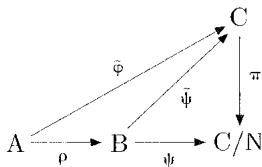
\includegraphics[keepaspectratio]{images/part001_4eedc660.jpg}}

Consider C and C/N as A-algebras by means of \(\tilde{\varphi}\), so that \(\psi\) is a homomorphism of \(A\) -algebras; since B is formally smooth over A, there exists a continuous homomorphism of A-algebras \(\tilde{\psi}: B \to C\) such that \(\pi \circ \tilde{\psi} = \psi\), whence a).

\begin{enumerate}
\def\labelenumi{\alph{enumi})}
\setcounter{enumi}{1}
\item
  It suffices to prove that the product of two formally smooth \(k\)-algebras \(\mathrm{A}_1\) and \(\mathrm{A}_2\) is formally smooth. Let \(\varphi : \mathrm{A}_1 \times \mathrm{A}_2 \to \mathrm{C} / \mathrm{N}\) be a continuous homomorphism of \(k\)-algebras. Set \(e_1 = \varphi(1,0)\), \(e_2 = \varphi(0,1)\), so that \(e_1\) and \(e_2\) are orthogonal idempotents in \(\mathrm{C} / \mathrm{N}\). Let \(\varphi_1 : \mathrm{A}_1 \to (\mathrm{C} / \mathrm{N})e_1\) and \(\varphi_2 : \mathrm{A}_2 \to (\mathrm{C} / \mathrm{N})e_2\) be the maps defined by \(\varphi_1(a_1) = \varphi(a_1,0)\) and \(\varphi_2(a_2) = \varphi(0,a_2)\); these are continuous homomorphisms of \(k\)-algebras, and one has \(\varphi(a_1,a_2) = \varphi_1(a_1) + \varphi_2(a_2)\) for every \((a_1,a_2) \in \mathrm{A}_1 \times \mathrm{A}_2\). There exists an idempotent element \(\tilde{e}_1\) of C such that \(\pi(\tilde{e}_1) = e_1\) (A, VIII, § 9, No. 4, Proposition 7); set \(\tilde{e}_2 = 1 - \tilde{e}_1\), so that \(\pi(\tilde{e}_2) = e_2\). To show that this holds for \(i = 1,2\), the homomorphism \(\mathrm{C}\tilde{e}_i \to (\mathrm{C} / \mathrm{N})e_i\) induced by \(\pi\) is surjective, with kernel \(\mathrm{N}\tilde{e}_i\); since the \(k\)-algebra \(\mathrm{A}_i\) is formally smooth, the homomorphism \(\varphi_i\) admits a continuous lifting \(\tilde{\varphi}_i\) to \(\mathrm{C}\tilde{e}_i\). The map \((a_1,a_2) \mapsto \tilde{\varphi}_1(a_1) + \tilde{\varphi}_2(a_2)\) is a continuous lifting of \(\varphi\) to C.
\item
  Let \(i: \mathrm{A} \to \widehat{\mathrm{A}}\) be the canonical homomorphism. For every ring D equipped with the discrete topology, the map that assigns to a continuous homomorphism \(f: \widehat{\mathrm{A}} \to \mathrm{D}\) the continuous homomorphism \(f \circ i: \mathrm{A} \to \mathrm{D}\) is bijective. Assertion c) follows from this.
\end{enumerate}

The assertion c) of the proposition applies in particular when the topology of \(A\) is the J-adic topology, where \(J\) is a finitely generated ideal: the closure \(\widehat{J}\) of \(J\) in \(\widehat{A}\) is then equal to \(\widehat{JA}\) and the topology of \(\widehat{A}\) is the topology \(\widehat{J}\)-adic (III, § 2, No. 12, Corollary 2 of Proposition 16). Consequently, it is equivalent to say that \(A\) is formally smooth for the J-adic topology or that its separated completion \(\widehat{A}\) is formally smooth for the J-adic topology.

PROPOSITION 4.--- Let k be a ring, A and B k-algebras, J an ideal of A, and K an ideal of B.

\begin{enumerate}
\def\labelenumi{\alph{enumi})}
\item
  Let S be a multiplicative subset of A and T a subset of k whose image in A is contained in S. If \(A\) is formally smooth over \(k\) for the J-adic topology, S \(^{-1}A\) is formally smooth over \(\mathrm{T}^{-1}k\) for the topology \(\mathrm{S}^{-1}\mathrm{J}\)-adic.
\item
  Let \(k'\) be a \(k\)-algebra. If A is formally smooth over \(k\) for the J-adic topology, the \(k'\)-algebra \(A_{(k')}\) is formally smooth over \(k'\) for the \(JA_{(k')}\)-adic topology.
\item
  Let I denote the ideal of A ⊗k B generated by the images of J ⊗k B and A ⊗k K. If A and B are formally smooth over k for the J-adic and K-adic topologies, respectively, then the k-algebra A ⊗k B is formally smooth for the I-adic topology.
\item
  Under the hypotheses of a), let C be a \(\mathrm{T}^{-1}k\)-algebra and N an ideal of square zero in C; endow C and C/N with the discrete topology and denote \(\pi : C \to C/N\) the canonical surjection. Let \(\varphi : S^{-1}A \longrightarrow C/N\) be a homomorphism of \(\mathrm{T}^{-1}k\)-algebras, continuous for the \(\mathrm{S}^{-1}\mathrm{J}\)-adic topology. Denote by i the canonical homomorphism from A into \(S^{-1}A\). The map \(\varphi \circ i\) is a homomorphism of k-algebras, continuous for the J-adic topology, hence admits a lifting \(\tilde{\varphi}_{0} : A \to C\). The elements of \(\tilde{\varphi}_{0}(S)\) are invertible modulo N, hence invertible since N is nilpotent. Consequently there exists a ring homomorphism \(\tilde{\varphi} : S^{-1}A \to C\) such that \(\tilde{\varphi} \circ i = \tilde{\varphi}_{0}\) (II, § 2, No. 1, Proposition 1); by Corollary 3 of Proposition 2 of loc. cit., \(\tilde{\varphi}\) is \(\mathrm{T}^{-1}k\)-linear. We have \(\pi \circ \tilde{\varphi} \circ i = \varphi \circ i\), whence \(\pi \circ \tilde{\varphi} = \varphi\) (loc. cit., Proposition 1), so that \(\tilde{\varphi}\) is a lifting of \(\varphi\).
\item
  Let us place ourselves under the hypotheses of b). Let C be a \(k'\)-algebra and N an ideal of square zero in C; endow C and C/N with the discrete topology. Let \(\varphi : \mathrm{A}_{(k')} \longrightarrow \mathrm{C/N}\) be a homomorphism of \(k'\)-algebras, continuous for the \(J\mathrm{A}_{(k')}\)-adic topology. Let \(i : \mathrm{A} \to \mathrm{A}_{(k')}\) denote the canonical homomorphism. The map \(\varphi \circ i\) is a homomorphism of \(k\)-algebras from A to C/N, continuous for the J-adic topology; if A is formally smooth over \(k\) for the J-adic topology, \(\varphi \circ i\) admits a lifting \(\tilde{\psi} : \mathrm{A} \to \mathrm{C}\). The homomorphism of \(k'\)-algebras \(\tilde{\varphi} : \mathrm{A}_{(k')} \longrightarrow \mathrm{C}\) deduced from \(\tilde{\psi}\) is a lifting of \(\varphi\).
\item
  We place ourselves under the hypotheses of c). The B-algebra A⊗ \(_{k}\) B is formally smooth for the J(A⊗ \(_{k}\) B)-adic topology by b), hence for the I-adic topology; moreover, the canonical homomorphism B → A⊗ \(_{k}\) B is continuous when B is equipped with the K-adic topology and A⊗ \(_{k}\) B with the I-adic topology. Assertion c) therefore follows from Proposition 3, a).
\end{enumerate}

\subsection{Examples of formally smooth algebras}

Let k be a ring.

\begin{enumerate}
\def\labelenumi{\arabic{enumi})}
\tightlist
\item
  Let P be a projective \(k\)-module. The symmetric \(k\)-algebra \(\mathbf{S}_k(\mathrm{P})\) is formally smooth for the discrete topology, and a fortiori for the topology defined by its grading. Indeed, for any \(k\)-algebra C and every ideal N of C, the algebra homomorphisms from \(\mathbf{S}_k(\mathrm{P})\) into C (resp. C/N) are in bijective correspondence with the \(k\)-linear maps from P into C (resp. C/N), and the canonical map \(\mathrm{Hom}_k(\mathrm{P},\mathrm{C}) \to \mathrm{Hom}_k(\mathrm{P},\mathrm{C}/\mathrm{N})\) is surjective.
\end{enumerate}

Therefore (Proposition 3, c)), the \(k\)-algebra \(\widehat{\mathbf{S}}_k(\mathrm{P}) = \prod_{n\geqslant 0}\mathbf{S}_k^n (\mathrm{P})\) is formally smooth (for the product topology of the discrete topologies on the \(\mathbf{S}_k^n (\mathrm{P}))\)); indeed, it is the completion of the \(k\)-algebra \(\mathbf{S}_k(\mathrm{P})\) for the topology defined by the grading.

\begin{enumerate}
\def\labelenumi{\arabic{enumi})}
\setcounter{enumi}{1}
\item
  For any family of indeterminates \(\mathbf{T} = (\mathrm{T}_i)_{i\in I}\), the \(k\)-algebra of polynomials \(k[\mathbf{T}]\) and the \(k\)-algebra of formal power series \(k[[\mathbf{T}]]\), endowed with its canonical topology, are formally smooth; this follows from Example 1. If \(k\) is a field, the purely transcendental extension \(k(\mathbf{T})\) is formally smooth (No. 2, Proposition 4 a)).
\item
  Let \(f \in k[\mathrm{T}]\) be a polynomial in one indeterminate. To say that the \(k\)-algebra \(k[\mathrm{T}]/(f)\) is formally smooth is to say that the following property is satisfied: for every \(k\)-algebra C and every ideal N of square zero in C, every root of \(f\) in C/N lifts to a root of \(f\) in C. This is the case when \(f\) and its derivative \(f'\) generate the unit ideal. Indeed, let \(\alpha\) be a root of \(f\) in C/N and let \(a\) be an element of C lifting \(\alpha\). Then \(f(a)\) belongs to N and consequently \(f'(a)\) is invertible in C; the element \(b = a - f'(a)^{-1}f(a)\) lifts \(\alpha\). Since \(f'(a)^{-1}f(a)\) is of square zero, we have
\end{enumerate}

\[
f (b) = f (a) - f ^ {\prime} (a) f ^ {\prime} (a) ^ {- 1} f (a) = 0.
\]

THEOREM 1 (I. S. Cohen). Let \(k\) be a field and \(K\) a separable extension of \(k\). Then \(K\) is a formally smooth \(k\)-algebra.

Let C be a \(k\)-algebra, N an ideal of square zero in C, \(\pi: \mathrm{C} \to \mathrm{C/N}\) the canonical homomorphism, and \(\varphi: \mathrm{K} \to \mathrm{C/N}\) a homomorphism of \(k\)-algebras. It remains to construct a lifting of \(\varphi\). We distinguish two cases.

\begin{enumerate}
\def\labelenumi{\Alph{enumi})}
\item
  Suppose first that k has characteristic 0. Consider the pairs \((\mathrm{K}^{\prime}, \tilde{\varphi}^{\prime})\), where \(K^{\prime}\) is a subextension of K and \(\tilde{\varphi}^{\prime}: K^{\prime} \to C\) is a lifting of the restriction of \(\varphi\) to \(K^{\prime}\). The set of these pairs, ordered by extension, is inductive; by Zorn's lemma (E, III, p.~20, th. 2), there exists a maximal pair \((\mathrm{K}^{\prime}, \tilde{\varphi}^{\prime})\). Let us prove that \(K^{\prime}\) is equal to K. Let \(x \in K - K^{\prime}\). If x is transcendental over \(K^{\prime}\), the \(K^{\prime}\)-algebra \(\mathrm{K}^{\prime}(x)\) is formally smooth (example 2). If x is algebraic over \(K^{\prime}\), its minimal polynomial \(f \in K^{\prime}[T]\) is relatively prime to its derivative (A, V, p.~37, prop. 4), and \(\mathrm{K}^{\prime}(x)\) identifies with the \(K^{\prime}\)-algebra \(\mathrm{K}^{\prime}[\mathrm{T}]/(f)\), which is therefore a formally smooth \(K^{\prime}\)-algebra (example 3). In both cases, \(\mathrm{K}^{\prime}(x)\) is formally smooth over \(K^{\prime}\), and there exists an extension of \(\tilde{\varphi}^{\prime}\) to \(\mathrm{K}^{\prime}(x)\) that lifts the restriction of \(\varphi\) to \(\mathrm{K}^{\prime}(x)\), contradicting the maximality of \((\mathrm{K}^{\prime}, \tilde{\varphi}^{\prime})\).
\item
  Suppose \(k\) has characteristic \(p \neq 0\). Consider the ring homomorphism F: C → C such that F(x) = x \(^{p}\); one has F(x) = 0 for x ∈ N, so that there exists a unique ring homomorphism λ: C/N → C such that λ ∘ π = F. One has π(λ(π(x))) = π(x \(^{p}\)) = π(x) \(^{p}\); since π is surjective, one therefore has π(λ(z)) = z \(^{p}\) for every element z of C/N. On the other hand, let f: K → K \(^{p}\) be the isomorphism y ↦ y \(^{p}\) and let f \(^{-1}\): K \(^{p}\) → K be the inverse isomorphism. Let g: K \(^{p}\) → C be the composite of the following ring homomorphisms
\end{enumerate}

\[
\mathrm{K} ^ {p} \xrightarrow {f ^ {- 1}} \mathrm{K} \xrightarrow {\varphi} \mathrm{C} / \mathrm{N} \xrightarrow {\lambda} \mathrm{C}.
\]

For every \(x \in K\), one has \(g(x^{p}) = \lambda(\varphi(x))\). Since \(\lambda(\alpha z) = \alpha^{p}\lambda(z)\) for \(\alpha \in k\) and \(z \in C/N\), the map \(g\) is \(k^{p}\)-linear. Since the extension \(K\) of \(k\) is separable, \(k(K^{p})\) is identified with \(k \otimes_{k^{p}} K^{p}\) (A, V, p.~119, remark); consequently there exists a unique homomorphism of \(k\)-algebras \(h: k(K^{p}) \to C\) which coincides with \(g\) on \(K^{p}\).

Let \((a_{i})_{i\in I}\) be a \(p\)-basis of K over \(k(\mathrm{K}^p)\) (A, V, p.~98, theorem 2); for every \(i\in I\), choose an element \(b_{i}\) of C such that \(\pi(b_{i})=\varphi(a_{i})\). One has \(h(a_{i}^{p})=g(a_{i}^{p})=\lambda(\varphi(a_{i}))=\lambda(\pi(b_{i}))=b_{i}^{p}\) for every \(i\in I\). By A, V, p.~94, remark, there exists a homomorphism of \(k\)-algebras \(\tilde{\varphi}:K\to C\), extending \(h\) and such that \(\tilde{\varphi}(a_{i})=b_{i}\) for every \(i\). One has \(\pi(\tilde{\varphi}(a_{i}))=\pi(b_{i})=\varphi(a_{i})\) for every \(i\), and \(\pi(\tilde{\varphi}(x^{p}))=\pi(h(x^{p}))=\pi(g(x^{p}))=\pi(\lambda(\varphi(x)))=\varphi(x^{p})\) for every \(x\in K\). One therefore has \(\pi\circ\tilde{\varphi}=\varphi\), which completes the proof.

COROLLARY.--- Let k be a field, K a separable extension of k, and A a linearly topologized K-algebra. If A is formally smooth over K, it is formally smooth over k.

This follows from the theorem and from prop. 3 a) of no. 2.

Remarks.- 1) Let \(k\) be a field. Every \(k\) -algebra that is étale (A, V, p.~28, def. 1) is formally smooth (loc. cit., p.~34, th. 4, d) and no. 2, prop. 3, b)).

\begin{enumerate}
\def\labelenumi{\arabic{enumi})}
\setcounter{enumi}{1}
\tightlist
\item
  We shall see below (cor. 2 of th. 2 of no. 5) that a field extension which is formally smooth is absolutely regular, hence separable (§ 6, no. 4, example 2).
\end{enumerate}

\subsection{Liftings of homomorphisms in complete filtered algebras}

Let \(k\) be a ring, C a \(k\)-algebra, \((C_n)_{n \in \mathbf{Z}}\) a decreasing filtration of C, compatible with the structure of \(k\)-algebra and such that \(C_0 = C\) (III, § 2, no. 1). Suppose C is separated and complete for the topology defined by this filtration, so that the canonical map \(C \to \varprojlim C / C_n\) is a homeomorphism (loc. cit., no. 6). Let \(m\) be an integer \(>0\). Let us denote \(\pi: C \to C / C_m\) the canonical surjection.

PROPOSITION 5.—Let A be a formally smooth linearly topologized \(k\)-algebra. Every continuous homomorphism of \(k\)-algebras \(\varphi: A \to \mathrm{C/C}_{m}\) admits a continuous lifting to C.

For every integer \(n > m\), let us denote \(\pi_n: \mathrm{C/C}_n \to \mathrm{C/C}_{n-1}\) the canonical surjection. Since C is identified with the projective limit of the \(\mathrm{C/C}_n\), it is equivalent to give a continuous lifting of \(\varphi\) to C or a family \((\varphi_n)_{n > m}\) of continuous homomorphisms of \(k\)-algebras \(\varphi_n: \mathrm{A} \to \mathrm{C/C}_n\), satisfying \(\pi_n \circ \varphi_n = \varphi_{n-1}\). This brings us back, by induction on \(m\), to proving the statement when \(\mathrm{C}_{m+1} = 0\). The ideal \(\mathrm{C}_m\) is then of square zero (since \(2m \geqslant m+1\)), whence the proposition, since A is formally smooth.

Example.—Let C be a \(k\)-algebra and N a nilpotent ideal of C. The proposition applies to the algebra C equipped with the N-adic filtration. If A is a formally smooth linearly topologized \(k\)-algebra, we obtain that every continuous homomorphism from A into the \(k\)-algebra C/N, endowed with the discrete topology, lifts to a continuous homomorphism from A into the \(k\)-algebra C, equipped with the discrete topology.

\subsection{Formally smooth quotients of algebras}

THEOREM 2.--- Let k be a ring, A a k-algebra, and J an ideal of A such that the k-algebra A/J is formally smooth. Endow A with the J-adic topology. The following conditions are equivalent:

\begin{enumerate}
\def\labelenumi{(\roman{enumi})}
\item
  the topological k-algebra A is formally smooth;
\item
  the \(A/\mathrm{J}\)-module \(\mathrm{J}/\mathrm{J}^2\) is projective and the canonical homomorphism (§ 5, no. 2)
\end{enumerate}

\[
\beta : \mathbf {S} _ {\mathrm{A/J}} (\mathrm{J} / \mathrm{J} ^ {2}) \rightarrow \operatorname{gr} _ {\mathrm{J}} (\mathrm{A})
\]

is bijective;

\begin{enumerate}
\def\labelenumi{(\roman{enumi})}
\setcounter{enumi}{2}
\tightlist
\item
  the A/J-module J/J \(^{2}\) is projective and there exists an isomorphism of topological k-algebras from the separated completion of A onto the completion of the graded algebra \(\mathsf{S}_{A/J}\) (J/J \(^{2}\)).
\end{enumerate}

If A is Noetherian, these conditions are also equivalent to:

\begin{enumerate}
\def\labelenumi{(\roman{enumi})}
\setcounter{enumi}{3}
\tightlist
\item
  the ideal J is completely secant.
\end{enumerate}

First observe that (iii) implies (i): indeed, under the hypotheses of (iii), the algebra \(\mathsf{S}_{\mathrm{A}/\mathrm{J}}(\mathrm{J}/\mathrm{J}^{2})\) , endowed with the topology associated with its grading, is formally smooth over A/J (no. 3, example 1), hence over k (no. 2, prop. 3, a)); assertion (i) then follows from prop. 3, c) of no. 2.

Let \(\widehat{\mathbf{A}}\) be the separated completion of the algebra A and \(\widehat{\mathbf{J}}\) the separated completion of J. The canonical homomorphism \(i: \mathbf{A} \to \widehat{\mathbf{A}}\) induces an isomorphism \(\mathrm{A} / \mathrm{J} \longrightarrow \widehat{\mathrm{A}} / \widehat{\mathrm{J}}\) (III, § 2, no. 12, formula (21)). Let \(\varphi: \mathrm{A} / \mathrm{J} \to \widehat{\mathrm{A}}\) be a lifting of this isomorphism (no. 4, prop. 5). Denote \(\lambda: \widehat{\mathrm{J}} \to \mathrm{J} / \mathrm{J}^2\) the surjection deduced from the canonical isomorphism \(\mathrm{J} / \mathrm{J}^2 \longrightarrow \widehat{\mathrm{J}} / \widehat{\mathrm{J}}^2\) (III, § 2, no. 12, formula (21)). Let \(a\) be an element of A, \(\bar{a}\) its class in \(\mathrm{A} / \mathrm{J}\), and let \(z\) be an element of \(\widehat{\mathrm{J}}\); one has \(\varphi(\bar{a}) \equiv i(a)\) (mod. \(\widehat{\mathrm{J}}\)), whence \(\varphi(\bar{a})z \equiv i(a)z\) (mod. \(\widehat{\mathrm{J}}^2\)) and \(\lambda(\varphi(\bar{a})z) = \lambda(i(a)z) = \bar{a}\lambda(z)\). In other words, \(\lambda\) is A/J-linear when one equips \(\widehat{\mathbf{J}}\) with the structure of an A/J-module induced by \(\varphi\).

Suppose that the homomorphism \(\lambda\) admits an A/J-linear section \(\sigma : J/J^{2} \longrightarrow \widehat{J}\). Let \(S\) be the \(k\)-graded algebra \(S_{A/J}(J/J^{2})\) and \(\widehat{S}\) its completion. Let

\[
\theta : \mathsf {S} \to \widehat {\mathsf {A}}
\]

the homomorphism of \(k\)-algebras such that \(\theta(x) = \varphi(x)\) for \(x\) in \(\mathbf{S}^0 = \mathrm{A}/\mathrm{J}\), and \(\theta(x) = \sigma(x)\) for \(x\) in \(\mathbf{S}^1 = \mathrm{J}/\mathrm{J}^2\). Since \(\theta\) maps \(\mathbf{S}^1\) into \(\widehat{\mathbf{J}}\), it maps \(\mathbf{S}^n\) into \(\widehat{\mathbf{J}}^n\) and therefore extends to a continuous homomorphism \(\widehat{\boldsymbol{\theta}}: \widehat{\mathbf{S}} \to \widehat{\mathbf{A}}\). The map \(\mathrm{gr}_1(\boldsymbol{\theta}): \mathrm{J}/\mathrm{J}^2 \longrightarrow \widehat{\mathrm{J}}/\widehat{\mathrm{J}}^2\) is the composite of \(\sigma\) with the canonical surjection \(\widehat{\mathrm{J}} \longrightarrow \widehat{\mathrm{J}}/\widehat{\mathrm{J}}^2\); since \(\sigma\) is a section of \(\lambda\), \(\mathrm{gr}_1(\boldsymbol{\theta})\) coincides with the canonical isomorphism from \(\mathrm{J}/\mathrm{J}^2\) onto \(\widehat{\mathrm{J}}/\widehat{\mathrm{J}}^2\). Consequently \(\mathrm{gr}(\boldsymbol{\theta}): \mathbf{S} \to \mathrm{gr}_{\widehat{\mathbf{J}}}(\widehat{\mathbf{A}})\) is the composite of the canonical surjection \(\beta\) with the canonical isomorphism \(\mathrm{gr}_\mathrm{J}(\mathrm{A}) \to \mathrm{gr}_{\widehat{\mathbf{J}}}(\widehat{\mathbf{A}})\) (III, § 2, no. 12, formula (22)).

Now let us prove the implication (ii)⇒(iii). Under hypothesis (ii), the A/J-module J/J² is projective, so λ admits an A/J-linear section; the homomorphism \(\widehat{\boldsymbol{\theta}}:\widehat{\mathbf{S}}\to\widehat{\mathbf{A}}\) associated with this section by the preceding construction induces, by hypothesis, an isomorphism on the associated graded modules, hence is bijective (III, § 2, no. 8, cor. 3 of th. 1), which proves (iii).

Let us prove (i)⇒(ii). Suppose the topological k-algebra A is formally smooth. First we prove that the A/J-module \(J/J^{2}\) is projective. Let M be an \(A/J\)-module and \(f:M\to J/J^{2}\) a surjective A/J-linear map; the goal is to prove that f admits an A/J-linear section.

Let \(\pi: A/J^{2} \to A/J\) be the canonical surjection. By Remark 1 of No. 2, there exists an isomorphism of \(k\)-algebras \(\psi: A/J \oplus J/J^{2} \longrightarrow A/J^{2}\) such that \(\pi(\psi(y,z)) = y\) and \(\psi(0,z) = z\) for \(y \in A/J\), \(z \in J/J^{2}\). Consider the \(k\)-algebra (A/J) \(\oplus M\) (No. 1, example) and the map \(u: (A/J) \oplus M \to A/J^{2}\) such that \(u(x,m) = \psi(x,f(m))\). This is a surjective homomorphism of \(k\)-algebras, whose kernel is the kernel of \(f\) in M, hence is nilpotent of square zero. The canonical surjection \(\rho: A \to A/J^{2}\) is continuous; since A is formally smooth as a topological \(k\)-algebra, there exists a homomorphism of \(k\)-algebras \(\tilde{\rho}: A \to (A/J) \oplus M\) such that \(u \circ \tilde{\rho} = \rho\). Since \(\mathrm{pr}_{1} = \pi \circ \psi = \pi \circ u\), one has \(\mathrm{pr}_{1} \circ \tilde{\rho} = \pi \circ u \circ \tilde{\rho} = \pi \circ \rho\), so that \(\mathrm{pr}_{1} \circ \tilde{\rho}\) is the canonical surjection of A onto A/J. We therefore have \(\tilde{\rho}(J) \subset M\) and consequently \(\tilde{\rho}(J^{2}) = 0\), so that \(\tilde{\rho}\) induces an A/J-linear map \(s: J/J^{2} \to M\). One has \(u \circ \tilde{\rho} = \rho\) and \(\mathrm{pr}_{2} \circ \psi^{-1} \circ u(y,m) = f(m)\) for \(y \in A/J\) and \(m \in M\). Let \(x \in J\), and let \(\bar{x}\) be its class in \(J/J^{2}\); one has \(f(s(\bar{x})) = f(\mathrm{pr}_{2}(\tilde{\rho}(x))) = \mathrm{pr}_{2}(\psi^{-1}(\bar{x})) = \bar{x}\). Thus \(s\) is a section of \(f\).

It remains to prove that the homomorphism \(\beta\) is injective. Since the A/J-module \(J/J^{2}\) is projective, \(\lambda\) admits an A/J-linear section; denote by \(\theta: S \to \widehat{A}\) the associated homomorphism. The homomorphism gr(θ) is identified with \(\beta\). Let \(m\) be an integer; denote by \(\Sigma_{m}\) the graded \(k\)-algebra quotient of \(S\) by the ideal \(\sum_{i > m} S^{i}\) and \(\theta_{m}: \Sigma_{m} \to A/J^{m+1}\) the homomorphism deduced from \(\theta\). The composite of \(\theta_{m}\) with the canonical surjection \(A/J^{m+1} \longrightarrow A/J\) is the canonical projection of \(\Sigma_{m}\) onto \(S^{0} = A/J\); consequently the kernel of \(\theta_{m}\) is a nilpotent ideal. By the example in no. 4, there exists a lifting \(\psi_{m}: A \to \Sigma_{m}\) of the canonical surjection \(A \to A/J^{m+1}\). Since the composite of \(\psi_{m}\) with the canonical projection from \(\Sigma_{m}\) onto A/J is the canonical surjection, \(\psi_{m}(J)\) consists of elements of degree \(>0\). By passing to the associated graded objects, we deduce from \(\psi_{m}\) a \(k\)-linear graded map gr(\(\psi_{m}\)): gr \(_{J}(A) \to \Sigma_{m}\) such that gr \(_{m}(\theta) \circ\) gr \(_{m}(\psi_{m}) = \text{Id}_{J^{m}/J^{m+1}}\). It follows that gr \(_{m}(\theta)\), hence also \(\beta_{m}\), is injective, which completes the proof of (ii).

Finally, when A is Noetherian, conditions (ii) and (iv) are equivalent (§ 5, no. 2, th. 1).

COROLLARY 1.--- Let \(k\) a field and A a \(k\) -local Noetherian algebra such that the extension \(\kappa_{A}\) of \(k\) Let it be separable. The following conditions are equivalent:

\begin{enumerate}
\def\labelenumi{(\roman{enumi})}
\item
  the \(k\) -algebra A is formally smooth for the topology \(\mathfrak{m}_{\mathrm{A}}\) -adic;
\item
  the ring A is regular;
\item
  the \(k\)-algebra A is absolutely regular (\(\S 6, \mathrm{n}^{\circ} 4\), def. 1);
\item
  the k-algebra \(\hat{A}\) is isomorphic to \(\kappa_{A}[[T_{1},\ldots,T_{n}]]\) , with \(n=\dim A\) .
\end{enumerate}

Conditions (ii) and (iii) are equivalent by Example 3 of § 6, No. 4, and amount to saying that the ideal \(\mathfrak{m}_{\mathrm{A}}\) is completely secant (VIII, § 5, no. 2, th. 1). Moreover, every ring isomorphism of \(\widehat{\mathrm{A}}\) on \(\kappa_{\mathrm{A}}[[\mathrm{T}_{1},\ldots,\mathrm{T}_{n}]]\) is bicontinuous, since these are local rings. Since the \(k\) -algebra \(\mathrm{A}/\mathfrak{m}_{\mathrm{A}}\) is formally smooth (no. 3, th. 1), the corollary follows from th. 2 applied with \(\mathrm{J}=\mathfrak{m}_{\mathrm{A}}\) .

COROLLARY 2.--- Let k be a field, A a Noetherian k-algebra, and J an ideal of A contained in the radical of A. Suppose the k-algebra A is formally smooth for the J-adic topology. Then it is absolutely regular.

Indeed, let \(k'\) be a finite extension of \(k\) and \(A'\) the A-algebra \(A_{(k')}\); it remains to prove that, for every maximal ideal \(\mathfrak{m}'\) of \(A'\), the Noetherian local ring \(A_{\mathfrak{m}'}'\) is regular. Now we have \(JA' \subset \mathfrak{m}'\): indeed, the inverse image of \(\mathfrak{m}'\) in A is a maximal ideal of A (V, § 2, no. 1, prop. 1), hence contains J. The \(k'\)-algebra \(A'\) is formally smooth for the \(JA'\)-adic topology (no. 2, prop. 4, b)), and the \(k'\)-algebra \(A_{\mathfrak{m}'}'\) is formally smooth for the \(JA_{\mathfrak{m}'}'\)-adic topology (no. 2, prop. 4, a)), hence also for the \(\mathfrak{m}'A_{\mathfrak{m}'}'\)-adic topology. Let \(k_0\) be the prime subfield of \(k'\). Then \(A_{\mathfrak{m}'}'\) is formally smooth over \(k_0\) for the \(\mathfrak{m}'A_{\mathfrak{m}'}'\)-adic topology (cor. of th. 1 of no. 3); since \(\kappa(\mathfrak{m}')\) is separable over \(k_0\), the ring \(A_{\mathfrak{m}'}'\) is regular (cor. 1).

COROLLARY 3.--- Let k be a ring and A a formally smooth k-algebra.

\begin{enumerate}
\def\labelenumi{\alph{enumi})}
\item
  The A-module \(\Omega_k(A)\) is projective.
\item
  Suppose that the ring A ⊗k A is Noetherian. Let μ : A ⊗k A → A be the homomorphism such that μ(x ⊗ y) = xy; then the ideal Ker(μ) is completely secant.
\end{enumerate}

The \(k\)-algebras A and \(\mathbf{A} \otimes_{k} \mathbf{A}\) are formally smooth (no. 2, prop. 4, c)), and A is isomorphic to the quotient of \(\mathbf{A} \otimes_{k} \mathbf{A}\) by the kernel I of \(\mu\). By definition, \(\Omega_{k}(\mathbf{A}) = \mathbf{I}/\mathbf{I}^{2}\). Thus a) and b) follow from th. 2.

\subsection{Extension of the base field in regular algebras (nonzero characteristic)}

Let \(k\) be a ring and \(\rho: A \to B\) a homomorphism of \(k\)-algebras. The homomorphism \(\rho\) induces an A-linear map \(\Omega(\rho): \Omega_k(A) \to \Omega_k(B)\), and consequently a B-linear map \(\Omega_0(\rho): B \otimes_A \Omega_k(A) \to \Omega_k(B)\) (A, III, p.~135). Let \(\mathbf{T} = (\mathrm{T}_i)_{i \in I}\) be a family of indeterminates, and \(\mathbf{t} = (t_i)_{i \in I}\) a family of elements of B; for every polynomial \(f = \sum_{\alpha \in \mathbf{N}^{(I)}} c_\alpha \mathbf{T}^\alpha\) of A{[} \(\mathbf{T}\) {]}, let us denote by \(d^{A} f(\mathbf{t})\) the element \(\sum_{\alpha} \mathbf{t}^\alpha \otimes dc_\alpha\) of \(B \otimes_A \Omega_k(A)\).

Lemma 1.—Suppose that the A-algebra B admits a generating family \(\mathbf{t} = (t_i)_{i\in I}\), subject to the relations \(f_\lambda \in \mathrm{A}[\mathbf{T}]\) (\(\lambda \in \Lambda\)). The B-linear homomorphism

\[
\psi : (\mathrm{B} \otimes_ {\mathrm{A}} \Omega_ {k} (\mathrm{A})) \oplus \mathrm{B} ^ {(\mathrm{I})} \longrightarrow \Omega_ {k} (\mathrm{B})
\]

defined by \(\psi(\alpha,(b_i)) = \Omega_0(\rho)(\alpha) + \sum_{i\in I}b_i\,dt_i\) is surjective; its kernel is generated by the elements \(n_{\lambda} = \left(d^{A}f_{\lambda}(\mathbf{t}),\left(\frac{\partial f_{\lambda}}{\partial\mathrm{T}_{i}}(\mathbf{t})\right)_{i\in I}\right)\) for \(\lambda \in \Lambda\).

Consider the sequence of B-modules and B-linear maps

\[
\mathrm{B} ^ {(\Lambda)} \xrightarrow {\varphi} (\mathrm{B} \otimes_ {\mathrm{A}} \Omega_ {k} (\mathrm{A})) \oplus \mathrm{B} ^ {(\mathrm{I})} \xrightarrow {\psi} \Omega_ {k} (\mathrm{B}) \longrightarrow 0,
\]

where \(\varphi\) is the homomorphism such that \(\varphi(e_{\lambda}) = n_{\lambda}\) ; it remains to show that this sequence is exact. By A, II, p.~36, th. 1, it suffices to prove that, for every B-module M, the sequence

\[
0 \to \operatorname{Hom} _ {\mathrm{B}} (\Omega _{k}(\mathrm{B}), \mathrm{M}) \xrightarrow {\operatorname{Hom}(\psi,1)} \operatorname{Hom} _{\mathrm{B}} ((\mathrm{B} \otimes_{\mathrm{A}} \Omega _{k}(\mathrm{A})) \oplus \mathrm{B}^{(\mathrm{I})}, \mathrm{M}) \xrightarrow {\operatorname{Hom}(\varphi,1)} \operatorname{Hom}_{\mathrm{B}}(\mathrm{B}^{(\Lambda)}, \mathrm{M})
\]

is exact. Given the universal property of the module of differentials (A, III, p.~134), this sequence identifies with

\[
0 \to \mathrm{D} _ {k} (\mathrm{B}, \mathrm{M}) \xrightarrow {\psi^ {\prime}} \mathrm{D} _ {k} (\mathrm{A}, \mathrm{M}) \oplus \mathrm{M} ^ {\mathrm{I}} \xrightarrow {\varphi^ {\prime}} \mathrm{M} ^ {\Lambda}
\]

where \(\psi^{\prime}(\mathrm{D}) = (\mathrm{D}\circ \rho,(\mathrm{D}(t_{i}))_{i\in I})\) and \(\varphi^{\prime}(\Delta,(m_{i})) = \big(f_{\lambda}^{\Delta}(\mathbf{t}) + \sum_{i}\frac{\partial f_{\lambda}}{\partial\mathrm{T}_{i}}(\mathbf{t})m_{i}\big)_{\lambda \in \Lambda}\) (in accordance with A, V, p.~121, for every polynomial \(f = \sum_{\alpha \in \mathbf{N}^{(I)}}c_{\alpha}\mathbf{T}^{\alpha}\) of A{[}T{]}, we denote \(f^{\Delta}(\mathbf{t})\) as the element \(\sum_{\alpha}\mathbf{t}^{\alpha}\Delta(c_{\alpha})\). Now the exactness of this sequence follows from loc. cit., prop. 1, taking into account that a derivation D : B → M is \(k\)-linear if and only if \(D\circ\rho\) is so.

Let A be a ring. There exists a unique structure of \(\mathbf{Z}\)-algebra on A; we simply denote \(\Omega(A)\) the A-module \(\Omega_{\mathbf{Z}}(\mathrm{A})\). If \(\rho : k \to \mathrm{A}\) is a ring homomorphism, we have a canonical exact sequence of A-modules (A, III, p.~136, prop. 21) \(\mathrm{A} \otimes_k \Omega(k) \to \Omega(\mathrm{A}) \to \Omega_k(\mathrm{A}) \to 0\).

Suppose that A contains a subfield, and let P be the prime subfield of A; then \(\Omega(\mathrm{P})\) is zero and the canonical homomorphism of A-modules \(\Omega(\mathrm{A}) \to \Omega_{\mathrm{P}}(\mathrm{A})\) is bijective. If moreover A has characteristic \(p \neq 0\) (which means by definition that \(p\) is a prime number, \(p1_{\mathrm{A}} = 0\), and \(1_{\mathrm{A}} \neq 0\)), then P is identified with \(\mathbf{F}_p\). Moreover, every derivation of A vanishes on the subring \(\mathbf{A}^p\); for every subring \(k\) of A contained in \(\mathbf{A}^p\) (and, in particular, for every perfect subfield \(k\) of A), the canonical map \(\Omega(\mathrm{A}) \to \Omega_k(\mathrm{A})\) is bijective.

Let A be a ring of characteristic \(p \neq 0\) and \((f_i)_{1 \leqslant i \leqslant n}\) a finite sequence of elements of A. Denote by \(A_n\) the quotient ring of the polynomial ring \(A[T_1, \ldots, T_n]\) by the ideal generated by the polynomials \(T_i^p - f_i\) , for \(1 \leqslant i \leqslant n\) .

Lemma 2.—Suppose the ring A is local and Noetherian. Then \(A_{n}\) is local and Noetherian. The following conditions are equivalent:

\begin{enumerate}
\def\labelenumi{(\roman{enumi})}
\item
  \(A_{n}\) is regular;
\item
  A is regular and the elements \(1 \otimes df_{i}\) of the \(\kappa_{A}\) -vector space \(\kappa_{A} \otimes_{A} \Omega(A)\) are linearly independent.
\end{enumerate}

The ring \(A_{n}\) is Noetherian (III, § 2, cor. 3 of th. 2). The A-module \(A_{n}\) is free, hence faithfully flat; if \(A_{n}\) is regular, then A is regular (§ 4, no. 5, prop. 8 b)). We shall reason by induction on n, the lemma being evident if n = 0.

\begin{enumerate}
\def\labelenumi{\Alph{enumi})}
\tightlist
\item
  Let us first treat the case n = 1, setting \(T_{1} = T\), \(f_{1} = f\). Let a denote the class of f in \(\kappa_{A}\) and distinguish two cases, according as a belongs or does not belong to \(\kappa_{A}^{p}\). If \(a \notin \kappa_{A}^{p}\), then the polynomial \(T^{p} - a\) is irreducible in \(\kappa_{A}\) (A, V, p.~24, lemma 1) and \(\kappa_{A} \otimes_{A} A_{1}\) is isomorphic to the field \(\kappa_{A}[T]/(T^{p} - a)\). The ideal \(m_{A}A_{1}\) of \(A_{1}\) is therefore maximal, so that the ring \(A_{1}\) is local (V, § 2, no. 1, prop. 1). If A is regular, \(A_{1}\) is regular (VIII, § 5, no. 1, prop. 1). According to A, V, p.~99, prop. 6, the element da of \(\Omega(\kappa_{A})\) is not zero; since it is the image under the canonical map \(\kappa_{A} \otimes_{A} \Omega(A) \to \Omega(\kappa_{A})\) of \(1 \otimes df\), the latter is not zero. This proves the lemma in this case.
\end{enumerate}

Now suppose that \(a\) belongs to \(\kappa_{\mathrm{A}}^{p}\). There therefore exists an element \(g\) of A such that \(f - g^{p} \in \mathfrak{m}_{\mathrm{A}}\). Set \(h = f - g^{p}\). Since \(\mathrm{T}^{p} - f = (\mathrm{T} - g)^{p} - h\), the A-algebra \(A_{1}\) is isomorphic to \(\mathrm{A}[\mathrm{T}] / (\mathrm{T}^{p} - h)\). According to VIII, § 5, no. 4, prop. 4, the ring \(A_{1}\) is local and, for it to be regular, it is necessary and sufficient that A be regular and that \(h\) not belong to \(\mathfrak{m}_{\mathrm{A}}^{2}\). Now, since \(\kappa_{A}\) is formally smooth over the prime field (no. 3, th. 1), the canonical map

\[
\bar {d}: \mathfrak {m} _ {\mathrm{A}} / \mathfrak {m} _ {\mathrm{A}} ^ {2} \to \kappa_ {\mathrm{A}} \otimes_ {\mathrm{A}} \Omega (\mathrm{A})
\]

is injective (no. 2, remark 1); but the image under \(\bar{d}\) of the class of \(h\) modulo \(\mathfrak{m}_{\mathrm{A}}^{2}\) is equal to \(1 \otimes dh = 1 \otimes d(f - g^{p}) = 1 \otimes df\). This proves the lemma in this second case and completes the proof of the case \(n = 1\).

\begin{enumerate}
\def\labelenumi{\Alph{enumi})}
\setcounter{enumi}{1}
\tightlist
\item
  Suppose \(n > 1\) . The ring \(\mathrm{A}_{1}\) is local and Noetherian by the case already treated. The \(\mathrm{A}_{1}\) -algebra \(\mathrm{A}_{n}\) is identified with the quotient of \(\mathrm{A}_{1}[\mathrm{T}_{2},\ldots ,\mathrm{T}_{n}]\) by the ideal generated by the \(\mathrm{T}_i^p -f_i\) , \(i\geqslant 2\) ; by the induction hypothesis, it is a local ring and condition (i) is equivalent to the conjunction of the following two conditions:
\end{enumerate}

(i') A \(_{1}\) is regular;

(i'\,') the elements \(1 \otimes df_2, \ldots, 1 \otimes df_n\) of the \(\kappa_{\mathrm{A}_1}\) -vector space \(\kappa_{\mathrm{A}_1} \otimes_{\mathrm{A}_1} \Omega(\mathrm{A}_1)\) are linearly independent.

But (i') is equivalent, as we have just seen, to

(ii') A is regular and the element \(1 \otimes df_{1}\) of the \(\kappa_{A}\)-vector space \(\kappa_{A} \otimes_{A} \Omega(A)\) is not zero.

By Lemma 1, the canonical homomorphism \(\mathrm{A}_{1} \otimes_{\mathrm{A}} \Omega(\mathrm{A}) \to \Omega(\mathrm{A}_{1})\) induces an isomorphism of \(((\mathrm{A}_{1} \otimes_{\mathrm{A}} \Omega(\mathrm{A})) / \mathrm{A}_{1}(1 \otimes df_{1})) \oplus \mathrm{A}_{1}\) onto \(\Omega(\mathrm{A}_{1})\), and consequently an injective homomorphism of \((\kappa_{\mathrm{A}_{1}} \otimes_{\mathrm{A}} \Omega(\mathrm{A})) / \kappa_{\mathrm{A}_{1}}(1 \otimes df_{1})\) into \(\kappa_{\mathrm{A}_{1}} \otimes_{\mathrm{A}_{1}} \Omega(\mathrm{A}_{1})\). Since \(\kappa_{\mathrm{A}_{1}} \otimes_{\mathrm{A}} \Omega(\mathrm{A})\) is identified with \(\kappa_{\mathrm{A}_{1}} \otimes_{\kappa_{\mathrm{A}}} (\kappa_{\mathrm{A}} \otimes_{\mathrm{A}} \Omega(\mathrm{A}))\), assertion (i'') is therefore equivalent to:

(ii'') the elements \(1 \otimes df_2, \ldots, 1 \otimes df_n\) are linearly independent in \((\kappa_{\mathrm{A}} \otimes_{\mathrm{A}} \Omega(\mathrm{A})) / \kappa_{\mathrm{A}}(1 \otimes df_1)\).

But the conjunction of (ii') and (ii'') is equivalent to (ii), which proves the lemma.

PROPOSITION 6. Let \(k\) be a field of characteristic \(p \neq 0\), \(k'\) be a radical extension of \(k\), of finite degree and height \(\leqslant 1\), and let A be a local regular \(k\)-algebra. Then \(\mathrm{A}_{(k')}\) is a local ring and the following conditions are equivalent:

\begin{enumerate}
\def\labelenumi{(\roman{enumi})}
\item
  the ring \(A_{(k')}\) is regular;
\item
  the \(\kappa_{A}\)-linear map
\end{enumerate}

\[
\kappa_ {\mathrm{A}} \otimes_ {k ^ {\prime p}} \Omega_ {k ^ {p}} (k ^ {\prime p}) \longrightarrow \kappa_ {\mathrm{A}} \otimes_ {\mathrm{A}} \Omega (\mathrm{A})
\]

deduced from the canonical injection \(k^{\prime p}\to \mathrm{A}\) is injective.

Indeed, let \((x_{i})_{i\in \mathrm{I}}\) be a finite \(p\)-basis of \(k'\) over \(k\) (A, V, p.~98); for all \(i\in \mathrm{I}\), set \(f_{i} = x_{i}^{p}\in k\). The \(k\)-algebra \(k'\) is identified with the quotient of \(k[(\mathrm{T}_i)_{i\in \mathrm{I}}]\) by the ideal generated by the polynomials \(\mathrm{T}_i^p - f_i\), hence the A-algebra \(\mathrm{A}_{(k')}\) is the quotient of \(\mathrm{A}[(\mathrm{T}_i)_{i\in \mathrm{I}}]\) by the ideal generated by the polynomials \(\mathrm{T}_i^p - f_i1_{\mathrm{A}}\).

Moreover, \((f_{i})_{i\in\mathrm{I}}\) is a p-basis of \(k^{\prime p}\) over \(k^{p}\), and the \(k^{\prime p}\)-vector space \(\Omega_{k^{p}}(k^{\prime p})\) has the family of \(df_{i}\) as a basis (A, V, p.~97, th. 1). Proposition 6 then follows from Lemma 2.

\subsection{A criterion for formally smooth local algebras}

PROPOSITION 7. Let \(k_{0}\) be a ring, \(k\) a \(k_{0}\)-algebra, A a \(k\)-algebra, and \(\mathfrak{m}\) a maximal ideal of A. We assume that \(k\) and A/\(\mathfrak{m}\) are formally smooth over \(k_{0}\). For A to be formally smooth over \(k\) for the \(\mathfrak{m}\)-adic topology, it is necessary and sufficient that the following two conditions be satisfied:

\begin{enumerate}
\def\labelenumi{(\roman{enumi})}
\item
  the canonical homomorphism \(\mathsf{S}_{\mathrm{A} / \mathfrak{m}}(\mathfrak{m} / \mathfrak{m}^{2})\to \mathrm{gr}_{\mathfrak{m}}(\mathrm{A})\) is bijective;
\item
  the A/m-linear map
\end{enumerate}

\[
\omega : \mathrm{A} / \mathfrak {m} \otimes_ {k} \Omega_ {k _ {0}} (k) \longrightarrow \mathrm{A} / \mathfrak {m} \otimes_ {\mathrm{A}} \Omega_ {k _ {0}} (\mathrm{A})
\]

deduced from the canonical map \(k \to A\) is injective.

Let \(d_{k}:k\to \Omega_{k_{0}}(k)\) and \(d_{\mathrm{A}}:\mathrm{A}\to \Omega_{k_0}(\mathrm{A})\) be the universal \(k_{0}\)-derivations.

Suppose first that A is formally smooth over \(k\) for the \(\mathfrak{m}\)-adic topology. Then A is formally smooth over \(k_{0}\) for the \(\mathfrak{m}\)-adic topology (\(n^{\circ} 2\), prop. 3, a)), which is equivalent to (i) (\(n^{\circ} 5\), th. 2). Moreover, the \(k_{0}\)-derivation \(\lambda \mapsto 1 \otimes d_{k}(\lambda)\) of \(k\) in \(A/\mathfrak{m} \otimes_{k} \Omega_{k_{0}}(k)\) can be extended to a \(k_{0}\)-derivation of A into \(A/\mathfrak{m} \otimes_{k} \Omega_{k_{0}}(k)\) (\(n^{\circ} 2\), remark 2). There therefore exists an A-linear map \(u: \Omega_{k_{0}}(A) \to A/\mathfrak{m} \otimes_{k} \Omega_{k_{0}}(k)\) such that \(u(d_{A}(\lambda 1_{A})) = 1 \otimes d_{k}(\lambda)\) for every \(\lambda \in k\). The \(A/\mathfrak{m}\)-linear map \(A/\mathfrak{m} \otimes_{A} \Omega_{k_{0}}(A) \longrightarrow A/\mathfrak{m} \otimes_{k} \Omega_{k_{0}}(k)\) deduced from \(u\) is a retraction of \(\omega\), which proves (ii).

Conversely, suppose conditions (i) and (ii) are satisfied. Then A is formally smooth over \(k_{0}\) for the \(\mathfrak{m}\)-adic topology (\(n^{\circ}5\), th. 2) and the A-module \(\Omega_{k_{0}}(A)\) is projective (\(n^{\circ}5\), cor. 3 of th. 2). Fix an integer \(r \geqslant 0\) and consider the map, linear over \(A/\mathfrak{m}^{r}\),

\[
\omega_ {r}: \mathrm{A} / \mathfrak {m} ^ {r} \otimes_ {k} \Omega_ {k _ {0}} (k) \longrightarrow \mathrm{A} / \mathfrak {m} ^ {r} \otimes_ {\mathrm{A}} \Omega_ {k _ {0}} (\mathrm{A})
\]

deduced from the canonical map \(k\to\mathrm{A}\). Let \((\lambda_{i})_{i\in\mathrm{I}}\) be a family of elements of \(k\) such that the \(d_{k}(\lambda_{i})\) form a basis of the \(k\)-vector space \(\Omega_{k_{0}}(k)\). By (ii), the elements \(1 \otimes d_{A}(\lambda_{i}1_{A})\) are linearly independent in A/m \(\otimes_{\mathrm{A}} \Omega_{k_0}(\mathrm{A})\). By II, § 3, no. 2, cor. 1 and 2 of prop. 5, the \(1 \otimes d_{A}(\lambda_{i}1_{A})\) form a basis of a direct summand of the A/m \(^{r}\)-module A/m \(^{r} \otimes_{\mathrm{A}} \Omega_{k_0}(\mathrm{A})\). There therefore exists a map, linear over A/m \(^{r}\),

\[
u _ {r}: \mathrm{A} / \mathfrak {m} ^ {r} \otimes_ {\mathrm{A}} \Omega_ {k _ {0}} (\mathrm{A}) \longrightarrow \mathrm{A} / \mathfrak {m} ^ {r} \otimes_ {k} \Omega_ {k _ {0}} (k)
\]

such that \(u_r(1 \otimes d_A(\lambda_i 1_A)) = 1 \otimes d_k(\lambda_i)\) for every \(i\) , hence \(u_r \circ \omega_r = \mathrm{Id}\) .

Let us now verify that A is formally smooth over \(k\) for the m-adic topology. Let C be a \(k\)-algebra, N an ideal of square zero in C, and \(\pi: C \to C/N\) the canonical surjection; endow C and C/N with the discrete topology. Let \(\varphi: A \to C/N\) be a continuous homomorphism of \(k\)-algebras. Since A is formally smooth over \(k_0\) for the m-adic topology, there exists a continuous homomorphism of \(k_0\)-algebras \(\tilde{\varphi}_0: A \to C\) such that \(\pi \circ \tilde{\varphi}_0 = \varphi\). According to Proposition 1 of No. 1, the homomorphisms of \(k_0\)-algebras \(\tilde{\varphi}: A \to C\) such that \(\pi \circ \tilde{\varphi} = \varphi\) are the maps \(x \mapsto v(d_A(x)) + \tilde{\varphi}_0(x)\), where \(v\) ranges over \(\mathrm{Hom}_{A}(\Omega_{k_0}(A), N)\). It remains to choose \(v\) so that \(\tilde{\varphi}\) is a homomorphism of \(k\)-algebras. The map \(\lambda \mapsto \lambda 1_C - \tilde{\varphi}_0(\lambda 1_A)\) is a \(k_0\)-derivation from \(k\) into N (loc. cit.), hence can be written \(h \circ d_k\) with \(h \in \mathrm{Hom}_k(\Omega_{k_0}(k), N)\).

Let us choose an integer \(r\) such that the kernel of \(\varphi\) contains \(\mathfrak{m}^r\). The A-module N is annihilated by \(\mathfrak{m}^r\), and it suffices to take for \(v\) the composite of the sequence of homomorphisms

\[
\Omega_ {k _ {0}} (\mathrm{A}) \longrightarrow \mathrm{A} / \mathfrak {m} ^ {r} \otimes_ {\mathrm{A}} \Omega_ {k _ {0}} (\mathrm{A}) \xrightarrow {u _ {r}} \mathrm{A} / \mathfrak {m} ^ {r} \otimes_ {k} \Omega_ {k _ {0}} (k) \xrightarrow {h ^ {\prime}} \mathrm{N},
\]

where \(h'\) is deduced from \(h\). Indeed, we have, for \(\lambda \in k\):

\[
v \left(d _ {\mathrm{A}} \left(\lambda 1 _ {\mathrm{A}}\right)\right) = h ^ {\prime} u _ {r} \left(1 \otimes d _ {\mathrm{A}} \left(\lambda 1 _ {\mathrm{A}}\right)\right) = h ^ {\prime} \left(1 \otimes d _ {k} (\lambda)\right) = h \left(d _ {k} (\lambda)\right) = \lambda 1 _ {\mathrm{C}} - \tilde {\varphi} _ {0} \left(\lambda 1 _ {\mathrm{A}}\right).
\]

Remark 1.—When A is Noetherian, condition (i) means that the local ring \(A_{\mathfrak{m}}\) is regular (VIII, § 5, no. 2, th. 1).

PROPOSITION 8. Let \(k\) be a field and A a Noetherian local \(k\)-algebra. The following conditions are equivalent:

\begin{enumerate}
\def\labelenumi{(\roman{enumi})}
\item
  A is formally smooth over \(k\) for the \(\mathfrak{m}_{A}\)-adic topology;
\item
  A is regular and the \(\kappa_{\mathrm{A}}\)-linear map
\end{enumerate}

\[
\omega : \kappa_ {\mathrm{A}} \otimes_ {k} \Omega (k) \longrightarrow \kappa_ {\mathrm{A}} \otimes_ {\mathrm{A}} \Omega (\mathrm{A})
\]

deduced from the canonical injection k → A is injective ;

\begin{enumerate}
\def\labelenumi{(\roman{enumi})}
\setcounter{enumi}{2}
\item
  A is absolutely regular;
\item
  for every radical extension \(k'\) of \(k\) , of finite degree and height \(\leqslant 1\) , the local ring \(A_{(k')}\) is regular.
\item
  (ii) \(\Leftrightarrow\) (i): it suffices to apply Proposition 7 and Remark 1 above, taking \(k_{0}\) to be the prime subfield of \(k\); indeed, \(k\) and \(\kappa_{\mathrm{A}}\) are formally smooth over \(k_{0}\) (\(n^{\circ}3\), cf. th. 1).
\end{enumerate}

(i)⇒(iii): this follows from cor. 2 of th. 2 (no. 5).

(iii)⇒(iv): this follows from def. 1 of § 6, no. 4.

If \(k\) is of characteristic 0, it follows from Corollary 1 of Theorem 2 (No. 5) that (iv) implies (i), whence the proposition in this case. Suppose \(k\) has characteristic \(p \neq 0\) and prove (iv)⇒(ii). Let \(k'\) be a radical extension of \(k\) of finite degree and height \(\leqslant 1\). If A and \(\mathrm{A}_{(k')}\) are regular, the canonical map \(\kappa_{\mathrm{A}} \otimes_{k'^{p}} \Omega_{k^{p}}(k'^{p}) \longrightarrow \kappa_{\mathrm{A}} \otimes_{\mathrm{A}} \Omega(\mathrm{A})\) is injective (No. 6, Proposition 6). By Theorem 1(b) of A, V, p.~97, applied to the extension \(k\) of \(k^{p}\), the \(k\)-vector space \(\Omega(k)\), which coincides with \(\Omega_{k^{p}}(k)\), is the increasing filtered union of the subspaces \(k \otimes_{k'^{p}} \Omega_{k^{p}}(k'^{p})\), where \(k'\) ranges over the finite radical extensions of \(k\) of height \(\leqslant 1\) contained in a fixed algebraic closure of \(k\). The assertion (ii) follows from this.

Remark 2.—Let \(k\) be a field and A a \(k\)-algebra such that the ring \(\mathrm{A}_{(k')}\) is regular for every radical extension \(k'\) of \(k\), of finite degree and height \(\leqslant 1\); then A is absolutely regular. Indeed, let \(k'\) be such an extension; for every maximal ideal \(\mathfrak{m}\) of A, the ring \(k'\otimes_k\mathrm{A}_{\mathfrak{m}}\) is identified with a ring of fractions of \(\mathrm{A}_{(k')}\), hence is regular. By Proposition 8 above and Proposition 6 of § 6, No. 4, the algebra A is absolutely regular.

\subsection{Existence of retractions for linear maps}

PROPOSITION 9. Let A be a ring, M a finitely generated A-module, N a projective A-module, and u : M → N an A-linear map.

\begin{enumerate}
\def\labelenumi{\alph{enumi})}
\tightlist
\item
  Let p be a prime ideal of A. The following conditions are equivalent:
\end{enumerate}

\begin{enumerate}
\def\labelenumi{(\roman{enumi})}
\item
  there exists \(f \in \mathrm{A} - \mathfrak{p}\) and \(v \in \operatorname{Hom}_{\mathrm{A}_f}(\mathrm{N}_f, \mathrm{M}_f)\) with \(v \circ u_f = \operatorname{Id}_{\mathrm{M}_f}\) ;
\item
  there exists \(v \in \operatorname{Hom}_{\mathrm{A}_{\mathfrak{p}}}(\mathrm{N}_{\mathfrak{p}}, \mathrm{M}_{\mathfrak{p}})\) with \(v \circ u_{\mathfrak{p}} = \operatorname{Id}_{\mathrm{M}_{\mathfrak{p}}}\);
\item
  the \(\kappa(\mathfrak{p})\text{-linear map }1 \otimes u : \kappa(\mathfrak{p}) \otimes_{\mathrm{A}} \mathrm{M} \to \kappa(\mathfrak{p}) \otimes_{\mathrm{A}} \mathrm{N}\) is injective;
\item
  there exists an integer \(m \geqslant 0\), elements \(x_{1}, \ldots, x_{m}\) of M, and linear forms \(y_{1}, \ldots, y_{m}\) on N such that the images of the \(x_{i}\) in \(\mathrm{M}_{\mathfrak{p}}\) generate the \(\mathrm{A}_{\mathfrak{p}}\)-module \(\mathrm{M}_{\mathfrak{p}}\) and \(\det(<y_{j}, u(x_{i})>) \notin \mathfrak{p}\);
\end{enumerate}

If condition (iv) is satisfied, we have \(m = [\kappa(\mathfrak{p}) \otimes_{\mathrm{A}} \mathrm{M} : \kappa(\mathfrak{p})]\) and the elements \(1 \otimes x_i\) form a basis of the \(\kappa(\mathfrak{p})\)-vector space \(\kappa(\mathfrak{p}) \otimes_{\mathrm{A}} \mathrm{M}\).

\begin{enumerate}
\def\labelenumi{\alph{enumi})}
\setcounter{enumi}{1}
\tightlist
\item
  The set U of prime ideals p of A satisfying the conditions in a) is an open subset of Spec(A), and the following conditions are equivalent:
\end{enumerate}

\begin{enumerate}
\def\labelenumi{(\roman{enumi})}
\item
  We have U = Spec(A);
\item
  U contains all maximal ideals of A;
\item
  there exists \(v \in \operatorname{Hom}_{\mathrm{A}}(\mathrm{N}, \mathrm{M})\) with \(v \circ u = \operatorname{Id}_{\mathrm{M}}\);
\item
  u is injective and Coker(u) is a projective A-module.
\end{enumerate}

Let us prove a).

(i)⇒(ii)⇒(iii): these implications are clear.

(iii)⇒(iv): Set \(m = [\kappa(\mathfrak{p}) \otimes_{\mathrm{A}} \mathrm{M} : \kappa(\mathfrak{p})]\) and let \((x_{1}, \ldots, x_{m})\) be a sequence of elements of M such that the elements \(1 \otimes x_{i}\) form a basis of the \(\kappa(\mathfrak{p})\)-vector space \(\kappa(\mathfrak{p}) \otimes_{\mathrm{A}} \mathrm{M}\). By Nakayama's lemma, the images of the \(x_{i}\) in \(M_{p}\) generate the \(A_{p}\)-module \(M_{p}\). If condition (iii) is satisfied, the elements \(1 \otimes u(x_{i})\) of the \(\kappa(\mathfrak{p})\)-vector space \(\kappa(\mathfrak{p}) \otimes_{\mathrm{A}} N\) are linearly independent.

There exists moreover an A-module \(N'\), an index set I, and an isomorphism of A-modules \(\theta : N \oplus N' \to \mathrm{A}^{(\mathrm{I})}\), from which one deduces an isomorphism of \(\kappa(\mathfrak{p})\)-vector spaces

\[
\overline {{{\theta}}}: (\kappa (\mathfrak {p}) \otimes_ {\mathrm{A}} N) \oplus (\kappa (\mathfrak {p}) \otimes_ {A} N ^ {\prime}) \rightarrow \kappa (\mathfrak {p}) ^ {(I)}.
\]

The elements \(t_i = \bar{\theta}(1 \otimes u(x_i), 0)\) of \(\kappa(\mathfrak{p})^{(I)}\) form a finite free family. There therefore exist elements \(\alpha_1, \ldots, \alpha_{m}\) of I such that one has \(\det(\mathrm{pr}_{\alpha_j}(t_i)) \neq 0\) ; the linear forms \(y_j : z \mapsto \mathrm{pr}_{\alpha_j}(\theta(z, 0))\) on N are suitable.

Suppose condition (iv) is satisfied. Denote \((a_{ij}) \in \mathbf{M}_m(\mathrm{A})\) the matrix of coefficients \(a_{ij} = \langle y_j, u(x_i)\rangle\). Let \(g\) be an element of \(\mathrm{A} - \mathfrak{p}\) such that the images of the \(x_i\) generate the \(\mathrm{A}_g\)-module \(\mathrm{M}_g\) (II, § 5, no. 1, prop. 2), and let \(f = g \det(a_{ij})\). Since \(\det(a_{ij})\) is invertible in \(\mathrm{A}_f\), the images of the elements \(u(x_i)\) in \(\mathrm{N}_f\) are linearly independent; consequently the images of the \(x_i\) in \(\mathrm{M}_f\) form a basis of this \(\mathrm{A}_f\)-module. This proves the last assertion of a). Let us now prove (i). Denote by \(w \in \operatorname{Hom}_{\mathrm{A}}(\mathrm{N}, \mathrm{M})\) the map \(z \mapsto \sum_{j} \langle y_j, z\rangle x_j\). One has

\[
w \circ u (x _ {i}) = \sum_ {j} a _ {i j} x _ {j};
\]

since the images of the \(x_{i}\) form a basis of \(M_{f}\) and the matrix \((a_{ij})\) is invertible in \(\mathbf{M}_{m}(\mathrm{A}_{f})\), the endomorphism \((w \circ u)_{f}\) of \(M_{f}\) is bijective, and the map \(v = (w \circ u)_{f}^{-1} \circ w_{f} \in \operatorname{Hom}_{\mathrm{A}_{f}}(\mathrm{N}_{f}, \mathrm{M}_{f})\) satisfies condition (i).

Let us prove b). The fact that U is open follows from condition (i) of a).

(iii)⇒(i)⇒(ii): this is clear.

(iv)⇒(iii): under the hypotheses of (iv), the sequence 0 → M \(\xrightarrow{u}\) N \(\longrightarrow\) Coker(u) → 0 is exact and split, whence (iii).

\begin{enumerate}
\def\labelenumi{(\roman{enumi})}
\setcounter{enumi}{1}
\tightlist
\item
  (ii) \(\Rightarrow\) (iv): introduce as above an isomorphism of A-modules \(\theta: \mathrm{N} \oplus \mathrm{N}' \to \mathrm{A}^{(\mathrm{I})}\). Let \(u'\) be the map from M to \(\mathrm{A}^{(\mathrm{I})}\) defined by \(u'(x) = \theta(u(x), 0)\). There exists a finite subset J of I such that the image of \(u'\) is contained in the submodule \(\mathrm{A}^{\mathrm{J}}\) of \(\mathrm{A}^{(\mathrm{I})}\). Let \(u'': \mathrm{M} \to \mathrm{A}^{\mathrm{J}}\) be the map induced by \(u'\). Under hypothesis (ii), for every maximal ideal m of A, the \(\mathrm{A}_{\mathfrak{m}}\)-linear map \(u_{\mathfrak{m}}'\) from \(\mathrm{M}_{\mathfrak{m}}\) into \(\mathrm{A}_{\mathfrak{m}}^{(\mathrm{I})}\) admits a retraction, and hence so does \(u_{\mathfrak{m}}''\); thus \(u_{\mathfrak{m}}''\) is injective and its image is a direct summand in \(\mathrm{A}_{\mathfrak{m}}^{\mathrm{J}}\), so that its cokernel is a projective \(\mathrm{A}_{\mathfrak{m}}\)-module. The A-module \(\operatorname{Coker}(u'')\) is of finite presentation by construction; it is therefore projective (II, § 5, no. 2, th. 1). The homomorphism \(u''\) is injective (II, § 3, no. 3, th. 1); consequently, \(u\) is injective. The A-module \(\operatorname{Coker}(u')\) is isomorphic, on the one hand, to \(\operatorname{Coker}(u) \oplus \mathrm{N}'\) and, on the other hand, to \(\operatorname{Coker}(u'') \oplus \mathrm{A}^{(\mathrm{I}-\mathrm{J})}\). Since the A-modules \(\mathrm{A}^{(\mathrm{I}-\mathrm{J})}\), \(\operatorname{Coker}(u'')\), and \(\mathrm{N}'\) are projective, it follows that \(\operatorname{Coker}(u)\) is projective, which completes the proof of (iv).
\end{enumerate}
